\chapter{
%Modeling Animal space-usage with
%Detection Models based on Ecological Distance
%Ecological Distance Models in Spatial Capture-Recapture
Modeling Landscape Connectivity in Spatial Capture-Recapture Models
}
\markboth{Ecological Distance}{}
\label{chapt.ecoldist}


\vspace{.3in}



Every spatial capture-recapture model that we have considered so far
has expressed encounter probability as function of the Euclidean
distance between individual activity
centers ${\bf s}$ and trap locations ${\bf x}$. 
As a practical matter, models based on Euclidean
distance imply circular, symmetric, and stationary home ranges of
individuals, and these are not often biologically realistic.
While these simple encounter
probability models will often
be sufficient for practical
purposes, especially in small data sets, sometimes developing more
complex models of the detection process as it relates to space usage
of individuals will be useful.  Animals may not judge distance in
terms of Euclidean distance but, rather, according to quality of local
habitat, landscape connectivity, perceived mortality risk, and other
considerations affecting movement behavior.
Moreover, because encounter probability and the distance
metric upon which it is based represent outcomes of individual
movements about their home range, ecologists might have explicit
hypotheses about how environmental variables affect the distance
metric, and it is therefore desirable to incorporate these hypotheses
directly into SCR models so that they may be formally evaluated
statistically.  


Assessing the impacts of habitat fragmentation and habitat loss on
population density and landscape connectivity are high priorities in
applied ecological research.  Landscape connectivity is defined as the
degree to which landscape structure impedes or facilitates movement
\citep{tischendorf_fahrig:2000} and is widely recognized to be an
important component of population viability
\citep{with_crist:1995}. Although much theory has been developed to
predict the effects of decreasing connectivity, few empirical studies
have been conducted to test these predictions due to the paucity of
formal methods for estimating connectivity parameters
\citep{cushman_etal:2010}. Instead, ecologists often rely on expert
opinion or \textit{ad hoc} methods of specifying connectivity values,
even in important applied settings
\citep{adriaensen_etal:2003,beier_etal:2008,zeller_etal:2012}. In
addition, no methods are available for simultaneously estimating
population density and connectivity parameters, in spite of theory
predicting interacting effects of density and connectivity on
population viability \citep{tischendorf_etal:2005,cushman_etal:2010}.
In this chapter, following \citet{royle_etal:2012ecol}, we provide a
framework for modeling landscape connectivity using SCR models, by
parameterizing models for encounter probability based on ``ecological
distance''.  A natural candidate framework for modeling ecological
distance is the least-cost path which is used widely in landscape
ecology for modeling connectivity, movement and gene flow
\citep{adriaensen_etal:2003,manel_etal:2003,mcrae_etal:2008}.  In
practical applications, variables that influence landscape
connectivity, or the effective cost of moving across the landscape,
include things like highways \citep[e.g.,][]{epps_etal:2005},
elevation \citep{cushman_etal:2006}, ruggedness
\citep{epps_etal:2007}, snow cover \citep{schwartz_etal:2009},
distance to escape terrain \citep{shirk_etal:2010}, range limitations
\citep{mcrae_beier:2007}, or distance from urban areas, highways,
human disturbance or other factors that animals might avoid.  Together
multiple environmental variables create a resistance surface, which
forms the linchpin of all connectivity planning
\citep{spear_etal:2010}.

Following \citet{royle_etal:2012ecol}, we adopt an SCR modeling
framework based on least-cost path. That is, we parameterize encounter
probability {\it not} based on Euclidean distance but, rather, based
on the least-cost path between an individual's activity center and a
trap location. This is parameterized in terms of one or more
parameters that relate the {\it resistance} of the landscape to
explicit covariates.  In this way, we can explicitly accommodate
landscape structure and account for connectivity of the landscape in
SCR models. For these models based on least-cost path, we use a
likelihood-based inference framework although, in principle,
development of a Bayesian inference framework should not be too
difficult although we have not pursued this.  Using this
methodological extension of SCR models, it is possible to make formal
statistical inferences about movement and connectivity from
capture-recapture studies that generate sparse individual encounter
history data without subjective prescription of resistance or cost
surfaces, which is commonly done in practice.  While we believe there
should be much ecological interest in developing SCR models that
account for landscape connectivity, it is also important for obtaining
more accurate estimates of density.  \citet{royle_etal:2012ecol}
showed that, under simple models of landscape connectivity (governed
by a single covariate), a misspecified model based on Euclidean
distance can produce substantial bias in estimates of $N$ and hence
density.

{\bf 
Benefit: ecological distance itself is a function of z(s). not good:
this is a purely phenomenological description of how landscape is
used. It is not an explicit movement model. In next chapter we talk
about RSFs as a framework for modeling space usage explicitly in SCR
models. 
}
\section{Shortcomings of Euclidean Distance Models}


In the standard SCR models  encounter probability is modeled as a function
of Euclidean distance. For example, using the binomial observation model
(Chapt. \ref{chapt.scr0}), let
$y_{ij}$ be individual- and trap specific binomial counts
with sample size $K$ and probabilities
$p_{ij}$. The Gaussian model is
\[
p_{ij} = p_{0} \exp(-  d_{ij}^2 
/(2\sigma^{2}) )
\]
where $d_{ij} = ||{\bf x}_{j}, {\bf s}_{i}||$ is Euclidean
distance. As usual, we will sometimes adopt the
log-scale parameterization based on 
$\log(p_{ij})= \alpha_{0} + \alpha_{1} d_{ij}^{2}$ where
where $\alpha_{0} = \log(p_{0})$ and $\alpha_{1} = -1/(2\sigma^2)$.

The main problem with the Euclidean distance metric in this encounter
probability model is
 that it is unaffected by
habitat or landscape structure, and it implies that the space used by
individuals is stationary and symmetric which may be unreasonable
assumptions for some species. By stationary here we mean in the formal
sense of
invariance to translation. That is, the properties of an individual
home range centered at some point ${\bf s}$ are exactly the same as
any other point say ${\bf s}'$.
As an example, if the common detection model based on a bivariate
normal probability distribution function is used, then the implied
space usage by {\it all} individuals, no matter their location in
space or local habitat conditions, is symmetric with circular contours
of usage intensity.

In the framework of \citet{royle_etal:2012ecol}, SCR models explicitly
incorporate information about the landscape so that a unit of distance
is variable depending on identified covariates, say $z({\bf x})$.
Thus, where an individual lives on the landscape, and the state of the
surrounding landscape, will determine the character of its usage of
space. In particular, they suggest distance metrics, based on
least-cost path, that imply irregular, asymmetric and non-stationary
home ranges of individuals. As an example, Fig. \ref{fig.distort}
shows a typical symmetric home range (left panel), and a compressed
home range (right panel) resulting from the effect of an environmental
variable (center panel)on an animal's movement behavior. We might
think of the environmental variable as representing an elevation
gradient of a valley and so, for a species that avoids high elevation,
space usage will be concentrated in flatter terrain at lower
elevations and therefore producing the elliptical home range shape.
We reproduce the application from \citet{royle_etal:2012ecol} later in
this chapter, in addition to providing an alternative applied context
that involves computing distances within odd-shaped landscape patches
(sec. \ref{ecoldist.sec.buffer}).


\begin{figure}[h]
\centering
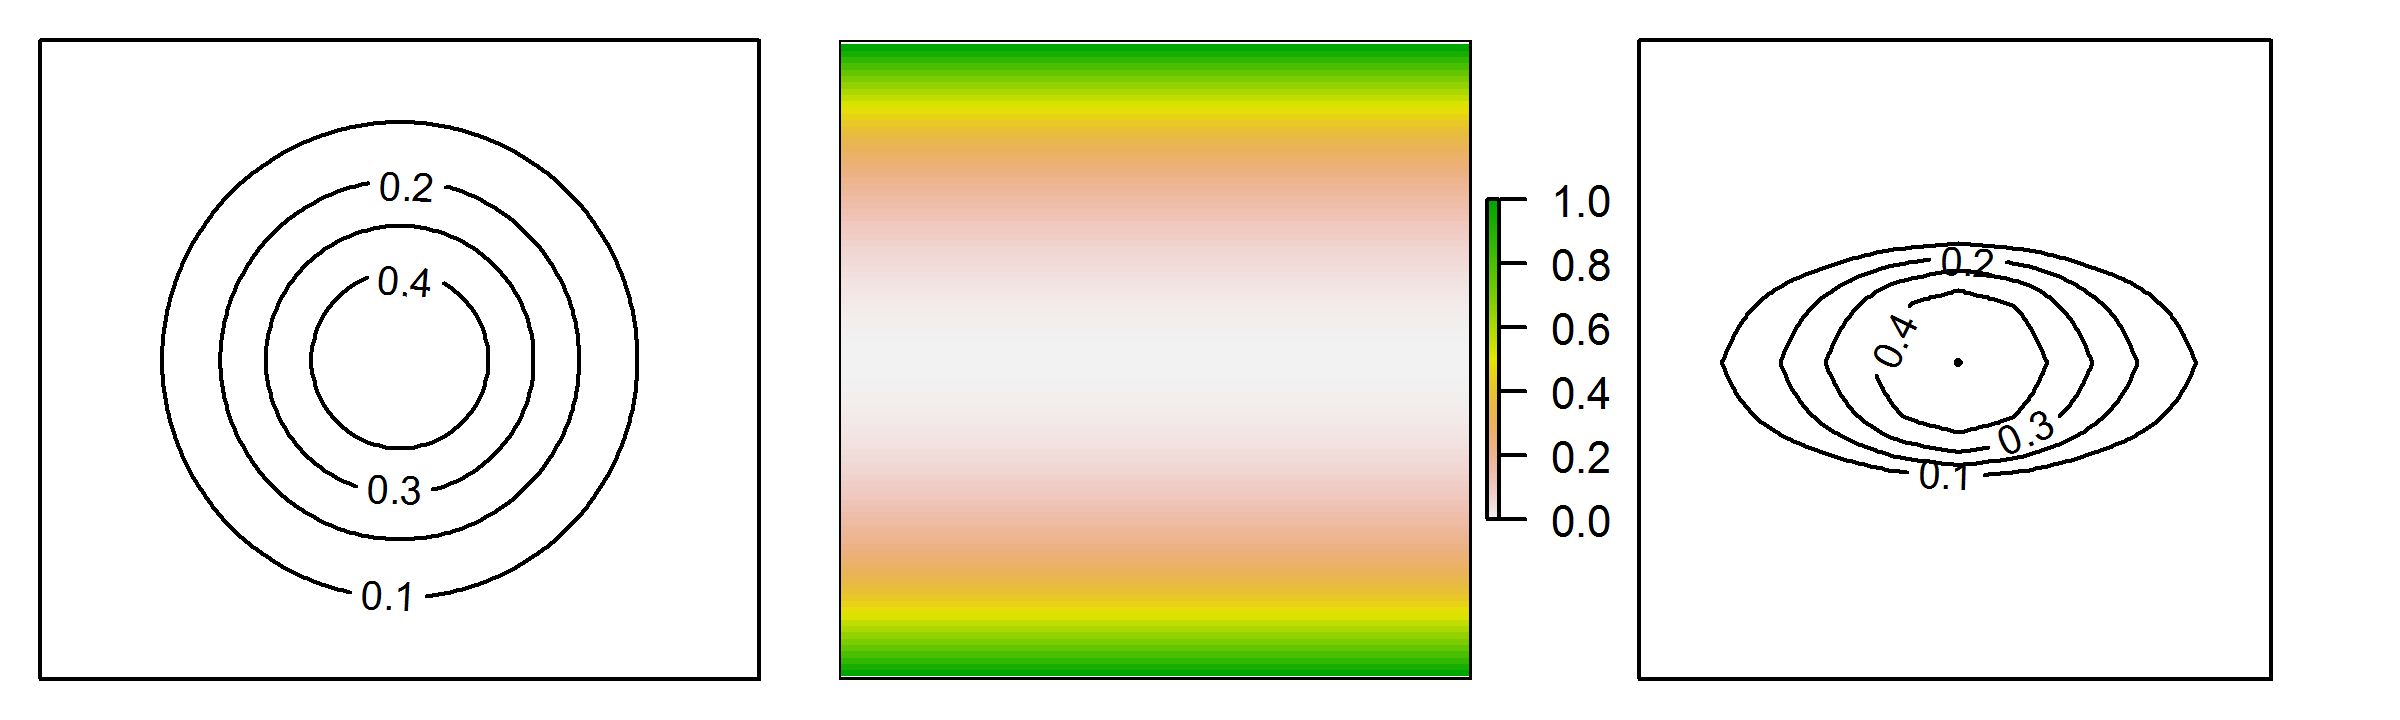
\includegraphics[width=5in,height=1.3in]{Ch10-EcolDist/figs/distort}
\caption{A symmetric home range (left), a habitat variable (center)
  such as representing an elevation gradient,
  and a non-symmetric home range (right) resulting from the cost imposed on
  movement by the habitat variable.}
\label{fig.distort}
\end{figure}


\section{Cost-Weighted Distance}

We adopt a cost-weighted distance metric here which defines
the effective distance between points by accumulating pixel-specific costs
determined using a cost function defined by the user.  The idea of
cost-weighted distance to characterize animal use of landscapes is
widely used in landscape ecology for modeling connectivity, movement
and gene flow \citep{beier_etal:2008}. For reasons of
computational tractability we consider a discrete landscape
defined by
a raster of some prescribed resolution. The distance between any two
points ${\bf x}$ and ${\bf x}'$ can be represented by a sequence of
line segments connecting neighboring pixels, say ${\bf l}_{1},{\bf
  l}_{2},\ldots,{\bf l}_{m}$. Then the cost-weighted distance between
${\bf x}$ and ${\bf x}'$ is
\begin{equation}
 d({\bf x},{\bf x}')
  =  \sum_{i=1}^{m-1} cost({\bf l}_{i},{\bf l}_{i+1})||{\bf l}_{i} - {\bf l}_{i+1}||
\label{eq.costweighted}
\end{equation}
where $cost({\bf l}_{i},{\bf l}_{i+1})$ is the user-defined cost 
to move
from pixel ${\bf l}_{i}$ to neighboring pixel ${\bf l}_{i+1}$ in the sequence.
Given the cost of each pixel, it is a simple matter to compute the
cost-weighted distance between any two pixels, along {\it any} path,
simply by accumulating the incremental  costs weighted by
distances.
In the context of
spatial capture-recapture models (and, more generally, landscape
connectivity) we are concerned with the {\it minimum} cost-weighted
distance, or the {\it least-cost path}, between any two points which
we will denote by $d_{lcp}$, which is
the
sequence ${\cal P} = ({\bf l}_{1},{\bf l}_{2},\ldots,{\bf l}_{m})$ that minimizes
the objective function defined by Eq. \ref{eq.costweighted}. That is,
\begin{equation}
 d_{lcp}({\bf x},{\bf x}')
  =  \min_{{\cal P}} \sum_{i=1}^{m-1} cost({\bf l}_{i},{\bf l}_{i+1})||{\bf l}_{i} - {\bf l}_{i+1}||
\label{eq.lcp}
\end{equation}
The least-cost path distance can be calculated in
 many geographic information systems and other software packages,
including the {\bf R} package \mbox{\tt
  gdistance} \citep{vanetten:2011} which we use below.

The key ecological aspect of least-cost path modeling is the
development
of models for pixel-specific cost.
In this paper we model cost as a function of one or more covariates
defined on every pixel of the according raster. For example, using a
single covariate $z({\bf x})$ we define the cost of moving from some pixel
${\bf x}$ to neighboring pixel ${\bf x}'$ as
\begin{equation}
\log(  cost({\bf x},{\bf x}'))=  \alpha_{2}\left( \frac{z({\bf
      x})+z({\bf x}')}{2}
\right)
\label{ecoldist.eq.cost}
\end{equation}
Thus, if $\alpha_{2} = 0$ then substituting $\mbox{cost}({\bf x},{\bf x}')
=\exp(0) = 1$ into
Eq. \ref{eq.lcp} will produce the ordinary Euclidean distance
between points. Here we assume the covariate $z$ is positive-valued
and constrain $\alpha_{2}\ge 0$ so as to avoid
negative costs. While not necessarily problematic from a mathematical
standpoint, negative costs are unrealistic biologically. 

The use of least-cost path models to model landscape connectivity has
been around for a long time. And, although $\alpha_{2}$ is rarely
known, conservation biologists design linkages that require this
resistance value as input \citep[see][and articles cited
therein]{beier_etal:2008}.  However, formal inference (e.g.,
estimation) of parameters is not often done.  Instead, in many
existing applications of least-cost path analysis, the parameter
$\alpha_{2}$ is fixed by the investigator, or based on expert opinion
\citep{beier_etal:2008}, although recently researchers have begun to
define costs based on resource selection functions, animal movement
\citep{tracy:2006, fortin_etal:2005}, or genetic distance data (e.g.,
\citet{gerlach_musolf:2000}; \citet{epps_etal:2007};
\citet{schwartz_etal:2009}. We address the integration of resource
selection models based on telemetry data with SCR models in Chapt. \ref{chapt.rsf}.

To formalize the use of cost-weighted distance in SCR models, we 
substitute Eq. \ref{eq.lcp} in the expression for encounter
probability (Eq. \ref{eq.encounter}) and maximize the resulting
likelihood which we address below. In doing so, we can directly 
estimate parameters of the least-cost path model, evaluate how 
landscape covariate influence connectivity, and test explicit hypotheses
about these things using only individual level encounter history data
from capture-recapture studies.




\subsection{Example of Computing Cost-weighted distance}

As an example of the cost-weighted distance calculation consider the
following landscape comprised of 16 pixels with unit spacing
identified as follows, along with the pixel-specific cost:
\begin{center}
\begin{verbatim}
         pixel ID                Cost
       1  5  9  13          100   1   1  1
       2  6 10  14          100 100   1  1
       3  7 11  15          100 100 100  1
       4  8 12  16          100 100   1  1
\end{verbatim}
\end{center}
This simple cost raster is shown in Fig. \ref{ecoldist.fig.raster}. We
assume the scale is such that the distance between neighboring pixels
in any cardinal direction is 1 unit, and the distance between
neighbors on a diagonal is $\sqrt{2}$ units.  We assigned low cost of
1 to ``good habitat'' pixels (or pixels we think of as ``highly
connected'' by virtue of being in good habitat) and, conversely, we
assign high cost (100) to ``bad habitat''. So the shortest
cost-weighted distance between pixels 5 and 9 in this example is just
1 unit, the shortest cost-distance between pixels 5 and 10 is
$\sqrt{2}(1+1)/2 = 1.414214$ units, the shortest distance between
pixels 4 and 8 is 100 units, while the shortest cost-distance between
4 and 12 is 150.5. A tough one is: what is the shortest distance
between 7 and 16? An individual at pixel 7 can move diagonal (which
has distance $\sqrt{2}$) and pay $sqrt(2)*(100+1)/2 + 1 =72.41778$.

\begin{figure}[h]
\begin{center}
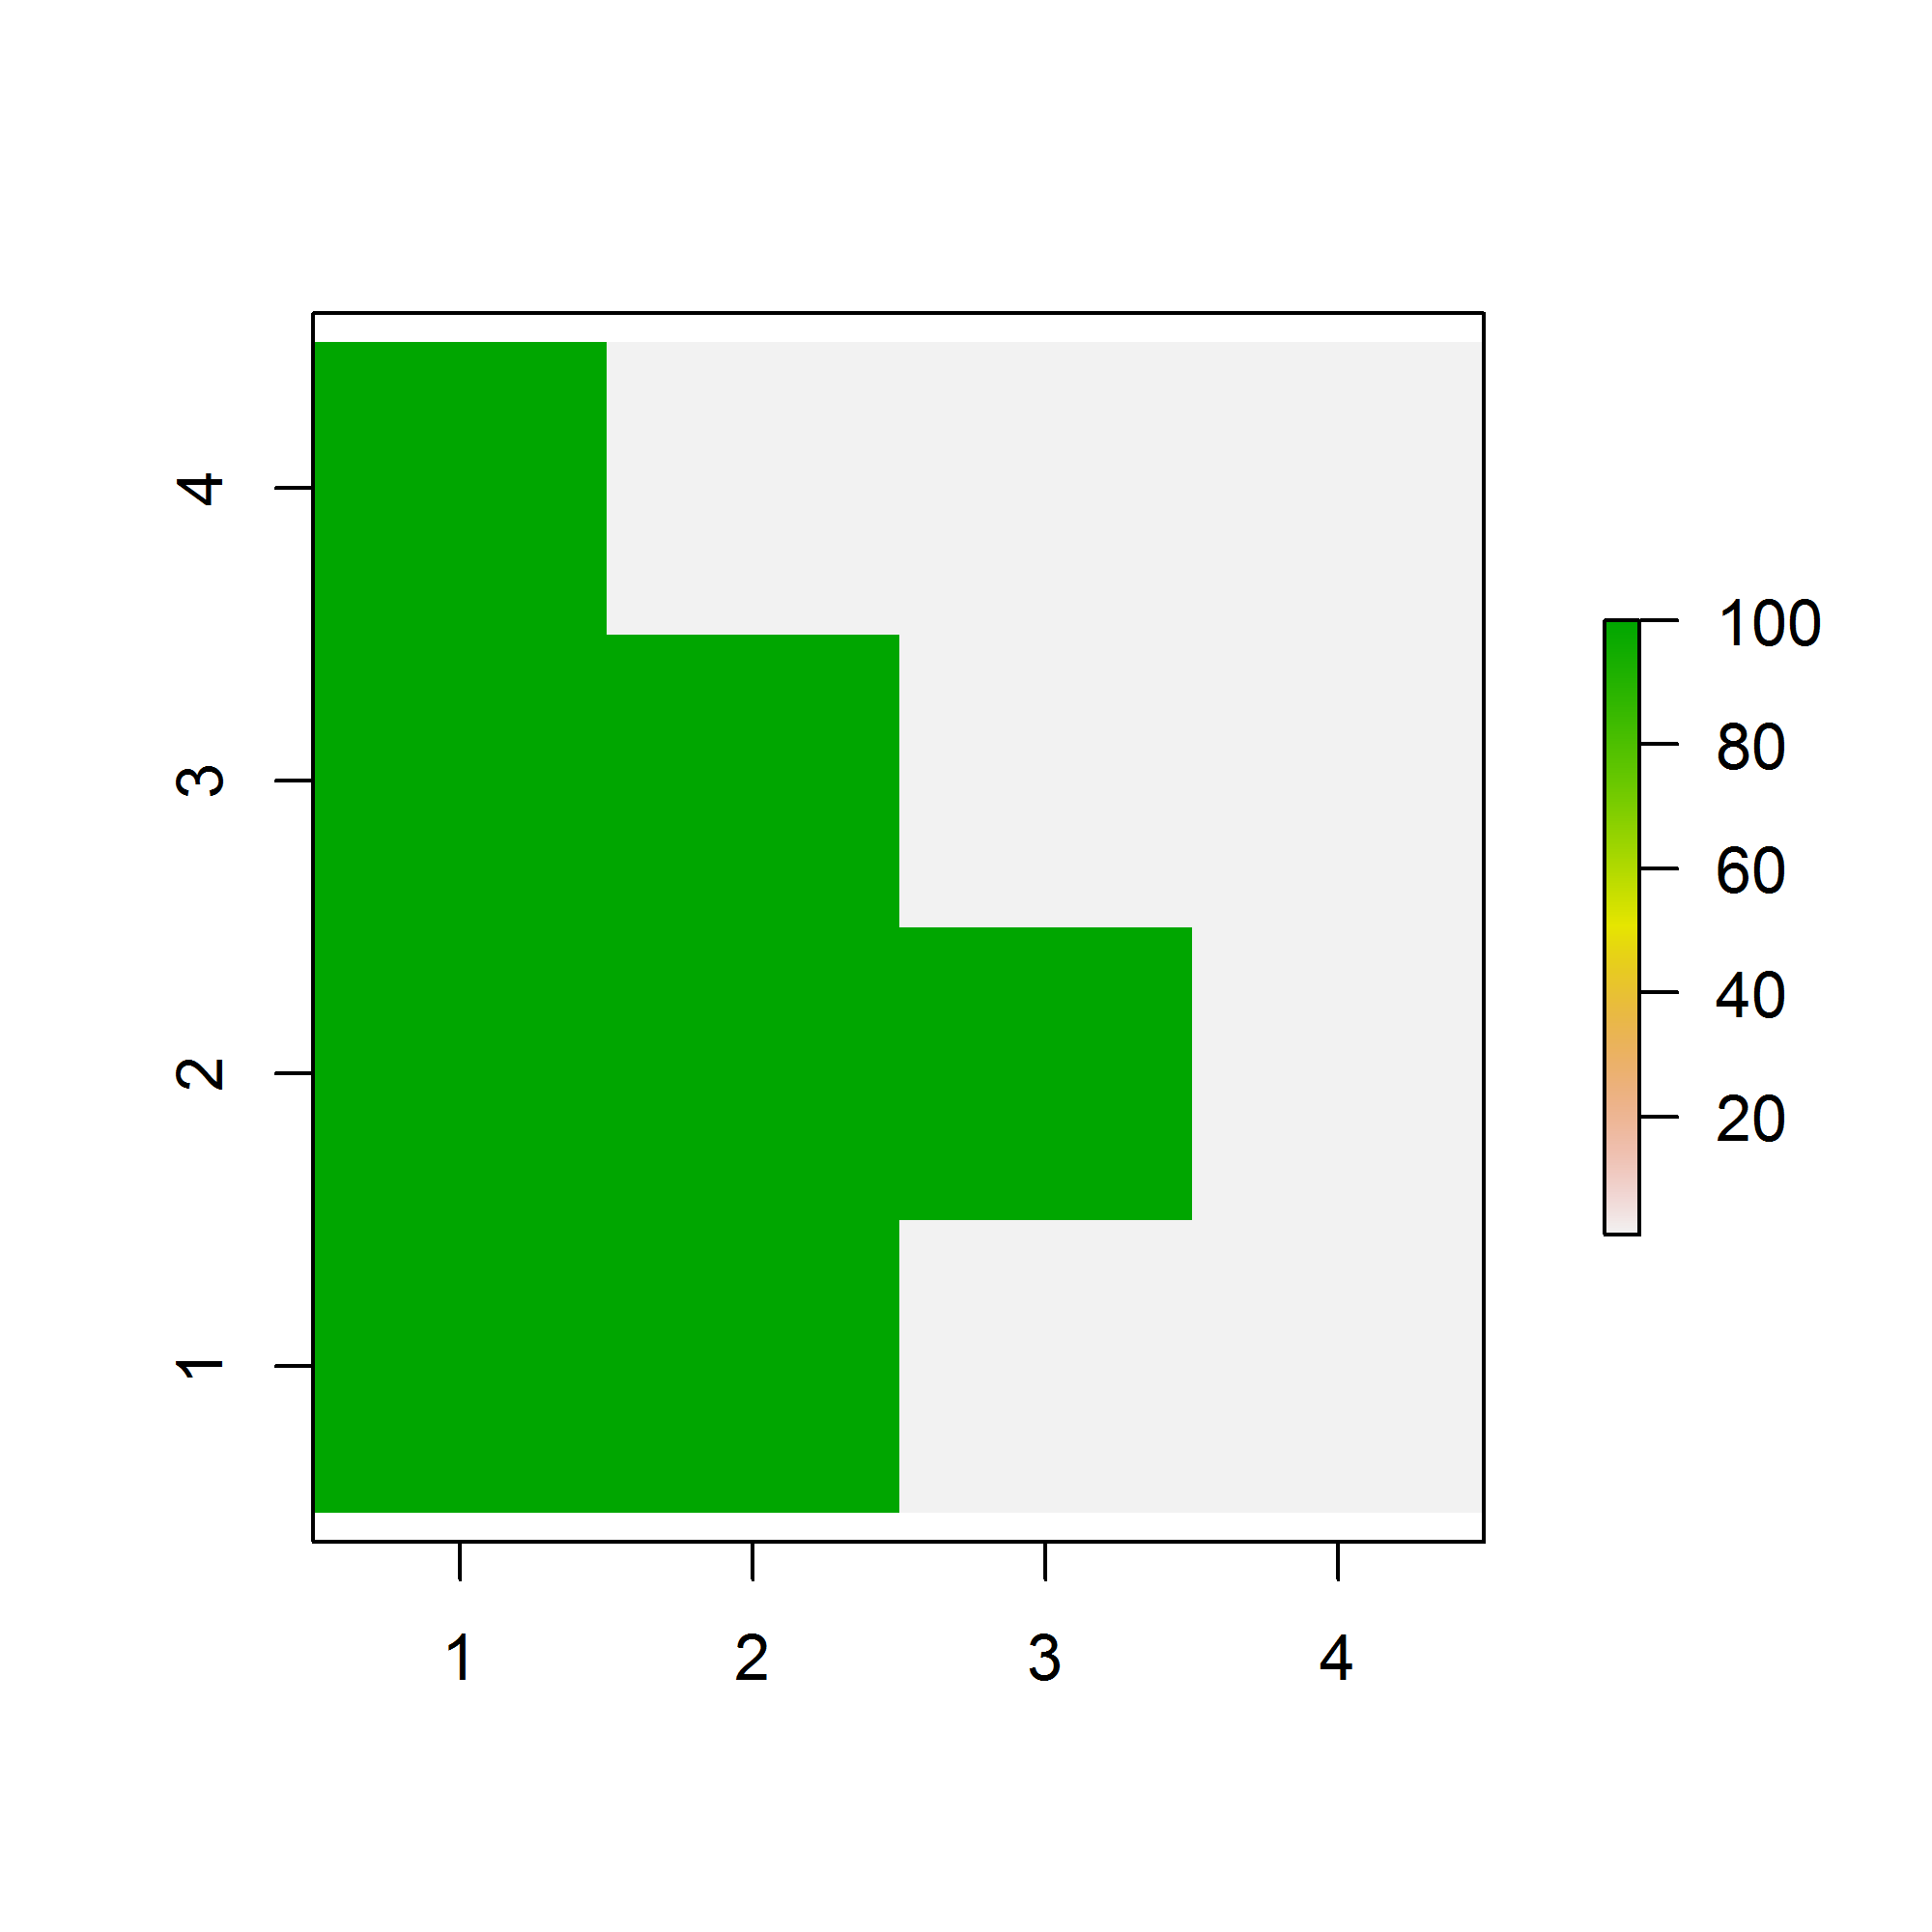
\includegraphics[height=3.25in,width=3.25in]{Ch10-EcolDist/figs/raster_2values}
\end{center}
\caption{A $4 \times 4$ raster depicting a binary cost surface, with cost = 1 (white) or 100 (shaded) to represent ease of movement across a pixel.}
\label{ecoldist.fig.raster}
\end{figure}

Once the cost raster is created, the least-cost path distances are
computed with just a couple {\bf R} commands, and those can be
inserted directly into the likelihood construction for an ordinary
spatial capture-recapture model The {\bf R} package
\mbox{\tt gdistance} calculates least-cost path using  Dijkstra's algorithm
\citep{dijkstra:1959} (from the \mbox{\tt igraph} package
\citep{csardi:2010}).  Using \mbox{\tt gdistance}, we 
define the incremental cost of moving from one pixel to another as the
distance-weighted {\it average} of the 2 pixel costs. We demonstrate
how to do this subsequently.

{\bf ANDY: Copy from revised appendix for the following material
  XXXXXXXXXXXX}

The {\bf R} commands for computing the least-cost distance between all pairs of pixels
are as follows:
\begin{verbatim}
r<-raster(nrows=4,ncols=4)
projection(r)<- "+proj=utm +zone=12 +datum=WGS84"
extent(r)<-c(.5,4.5,.5,4.5)
costs1<- c(100,100,100,100,1,100,100,100,1,1,100,1,1,1,1,1)
values(r)<-matrix(costs1,4,4,byrow=FALSE)
par(mfrow=c(1,1))
plot(r)
\end{verbatim}
Then we use the functions \mbox{\tt transition}, \mbox{\tt
  geoCorrection} {\bf XXX do we need this? XXXX}
 (which is only necessary if the data are not
projected or if cells are considered to have more than 4 neighbors)
 and \mbox{\tt costDistance} to compute the distance
matrix. The transition function computes the cost of making a
transition between
any two pixels, and it operates on the inverse-scale (''conductance'')
and so the
\mbox{\tt transitionFunction} argument is given as $1/mean(x)$.
To compute the cost distance we prescribe a set of points, or  we
can compute it  between
two sets of points (which is handy when one of the sets is of trap
locations, and the other is of individual activity centers).
To compute the distances for pixels in a raster,
we use the center points of each raster.  The {\bf R}
 commands altogether are as follows:
{\small
\begin{verbatim}
tr1<-transition(r,transitionFunction=function(x) 1/mean(x),directions=8)
tr1CorrC<-geoCorrection(tr1,type="c",multpl=FALSE,scl=FALSE)
pts<-cbind( sort(rep(1:4,4)),rep(4:1,4))
costs1<-costDistance(tr1CorrC,pts)
outD<-as.matrix(costs1)
\end{verbatim}
}
Now we can look at the result and see if it makes sense to us. Here we
produce the first 5 columns of this distance matrix to illustrate a
couple of examples of calculating the minimum cost-weighted distance
between points:
\begin{center}
{\small
\begin{verbatim}
> outD[1:5,1:5]
         1         2        3        4         5
1   0.0000 100.00000 200.0000 205.2426  50.50000
2 100.0000   0.00000 100.0000 200.0000  71.41778
3 200.0000 100.00000   0.0000 100.0000 171.41778
4 205.2426 200.00000 100.0000   0.0000 154.74264
5  50.5000  71.41778 171.4178 154.7426   0.00000
\end{verbatim}
}
\end{center}
An interesting case is that between point 1 and 4. Note that simply
taking the shortest Euclidean distance, weighted by cost, produces a
cost-weighted distance of $100 \times 1$ to move from pixel 1 to pixel
2, and similarly from 2 to 3 and 3 to 4, producing a total
cost-weighted distance of $300$. However, the actual {\it least-cost
  path} has cost-weighted distance $205.2426$ which 
 has an individual moving from pixel 1 to 5, then 5
to 10, 10 to 15, 15 to 12, 12 to 8 and 8 to 4, adding up to a cost
weighted distance of 
$205.2426$.


\section{Simulating SCR Data using Ecological Distance}
\label{ecoldist.sec.simulating}

\citet{royle_etal:2012ecol} simulated data based on two hypothetical
landscapes typical of how
cost-weighted distance models might be used in real capture-recapture
problems.  They defined a $20 \times 20$ pixel covariate raster with
extent = $[0.5, 4.5] \times [0.5, 4.5]$ which we imagine to be a 
 coarse landscape covariate, with pixels
having some arbitrary scaling. For example, think of each pixel as
representing, say, a $1 \times 1$ km grid cell in which case 
the raster defines a landscape of $20 \times 20$ km. We suppose
that 16 camera traps are established at the integer coordinates
$(1,1), (1,2), \ldots, (4,4)$. We could think of this as a landscape
within which we're studying a population of ocelots, lynx or some
other cat.

For our analyses here, we characterize cost by one covariate, 
and we consider two specific cases. First is an increasing trend from
the NW to the SE (''systematic covariate''), where $z({\bf x})$ is defined as
$z({\bf x}) = r({\bf x}) + c({\bf x})$ and $r({\bf x})$ and $c({\bf x})$ are just the row and
column, respectively, of the raster.  This might mimic something
related to distance from an urban area or a gradient in habitat
quality due to land use, or environmental conditions such as
temperature or precipitation gradients.  In the second case we make up
a covariate by generating a field of spatially correlated noise to
emulate a typical patchy habitat covariate (``patchy covariate'') such as
tree or understory density. The two covariates are shown in
Fig. \ref{ecoldist.fig.raster100}, along with a sample realization of
$N=100$ individuals (left panel only).  For both covariates we use a
cost function in which transitions from pixel ${\bf x}$ to ${\bf x}'$
is given by:
\[
 log(cost({\bf x},{\bf x}'))=  \alpha_2 \frac{z({\bf x}) + z({\bf x}')}{2}
\]
where $\alpha_2 = 1$ for simulating the observed data.
 Remember that with $\alpha_2=0$ the
model reduces to one in which the cost of moving across each pixel is
constant, and therefore Euclidean distance is operative.

\begin{figure}[h]
\begin{tabular}{ll}
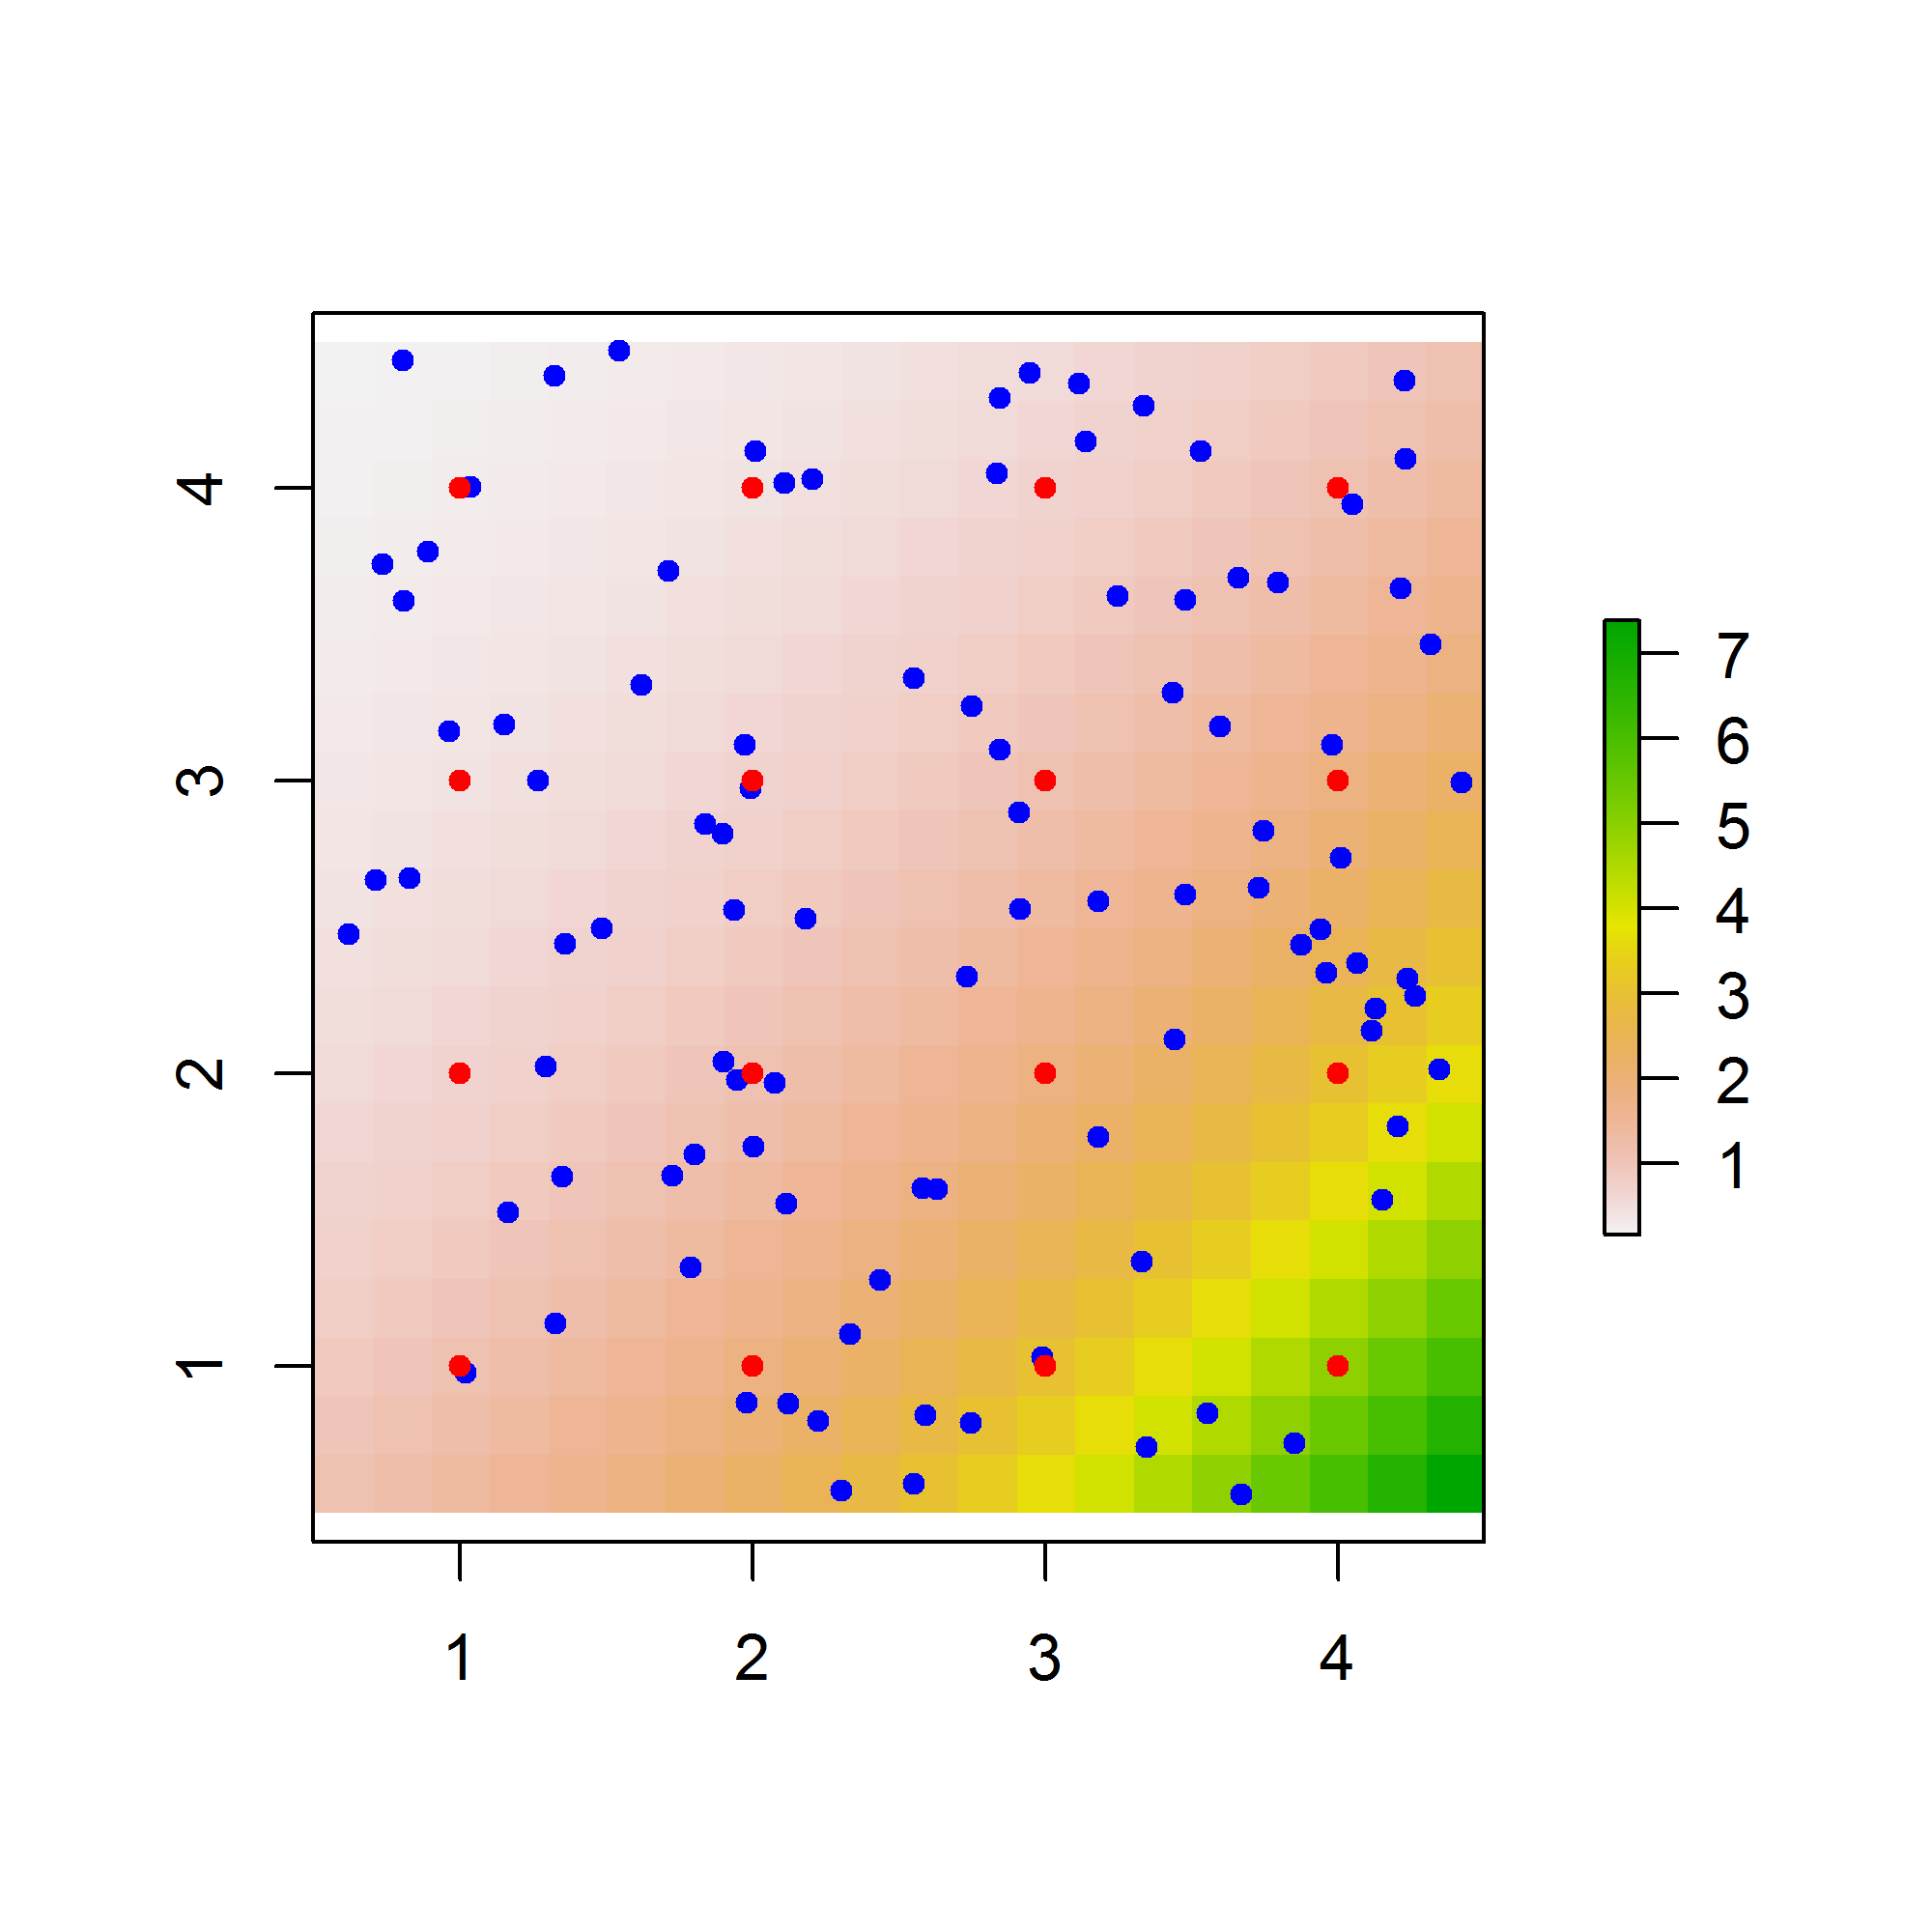
\includegraphics[height=2.5in,width=2.5in]{Ch10-EcolDist/figs/raster_withN100}
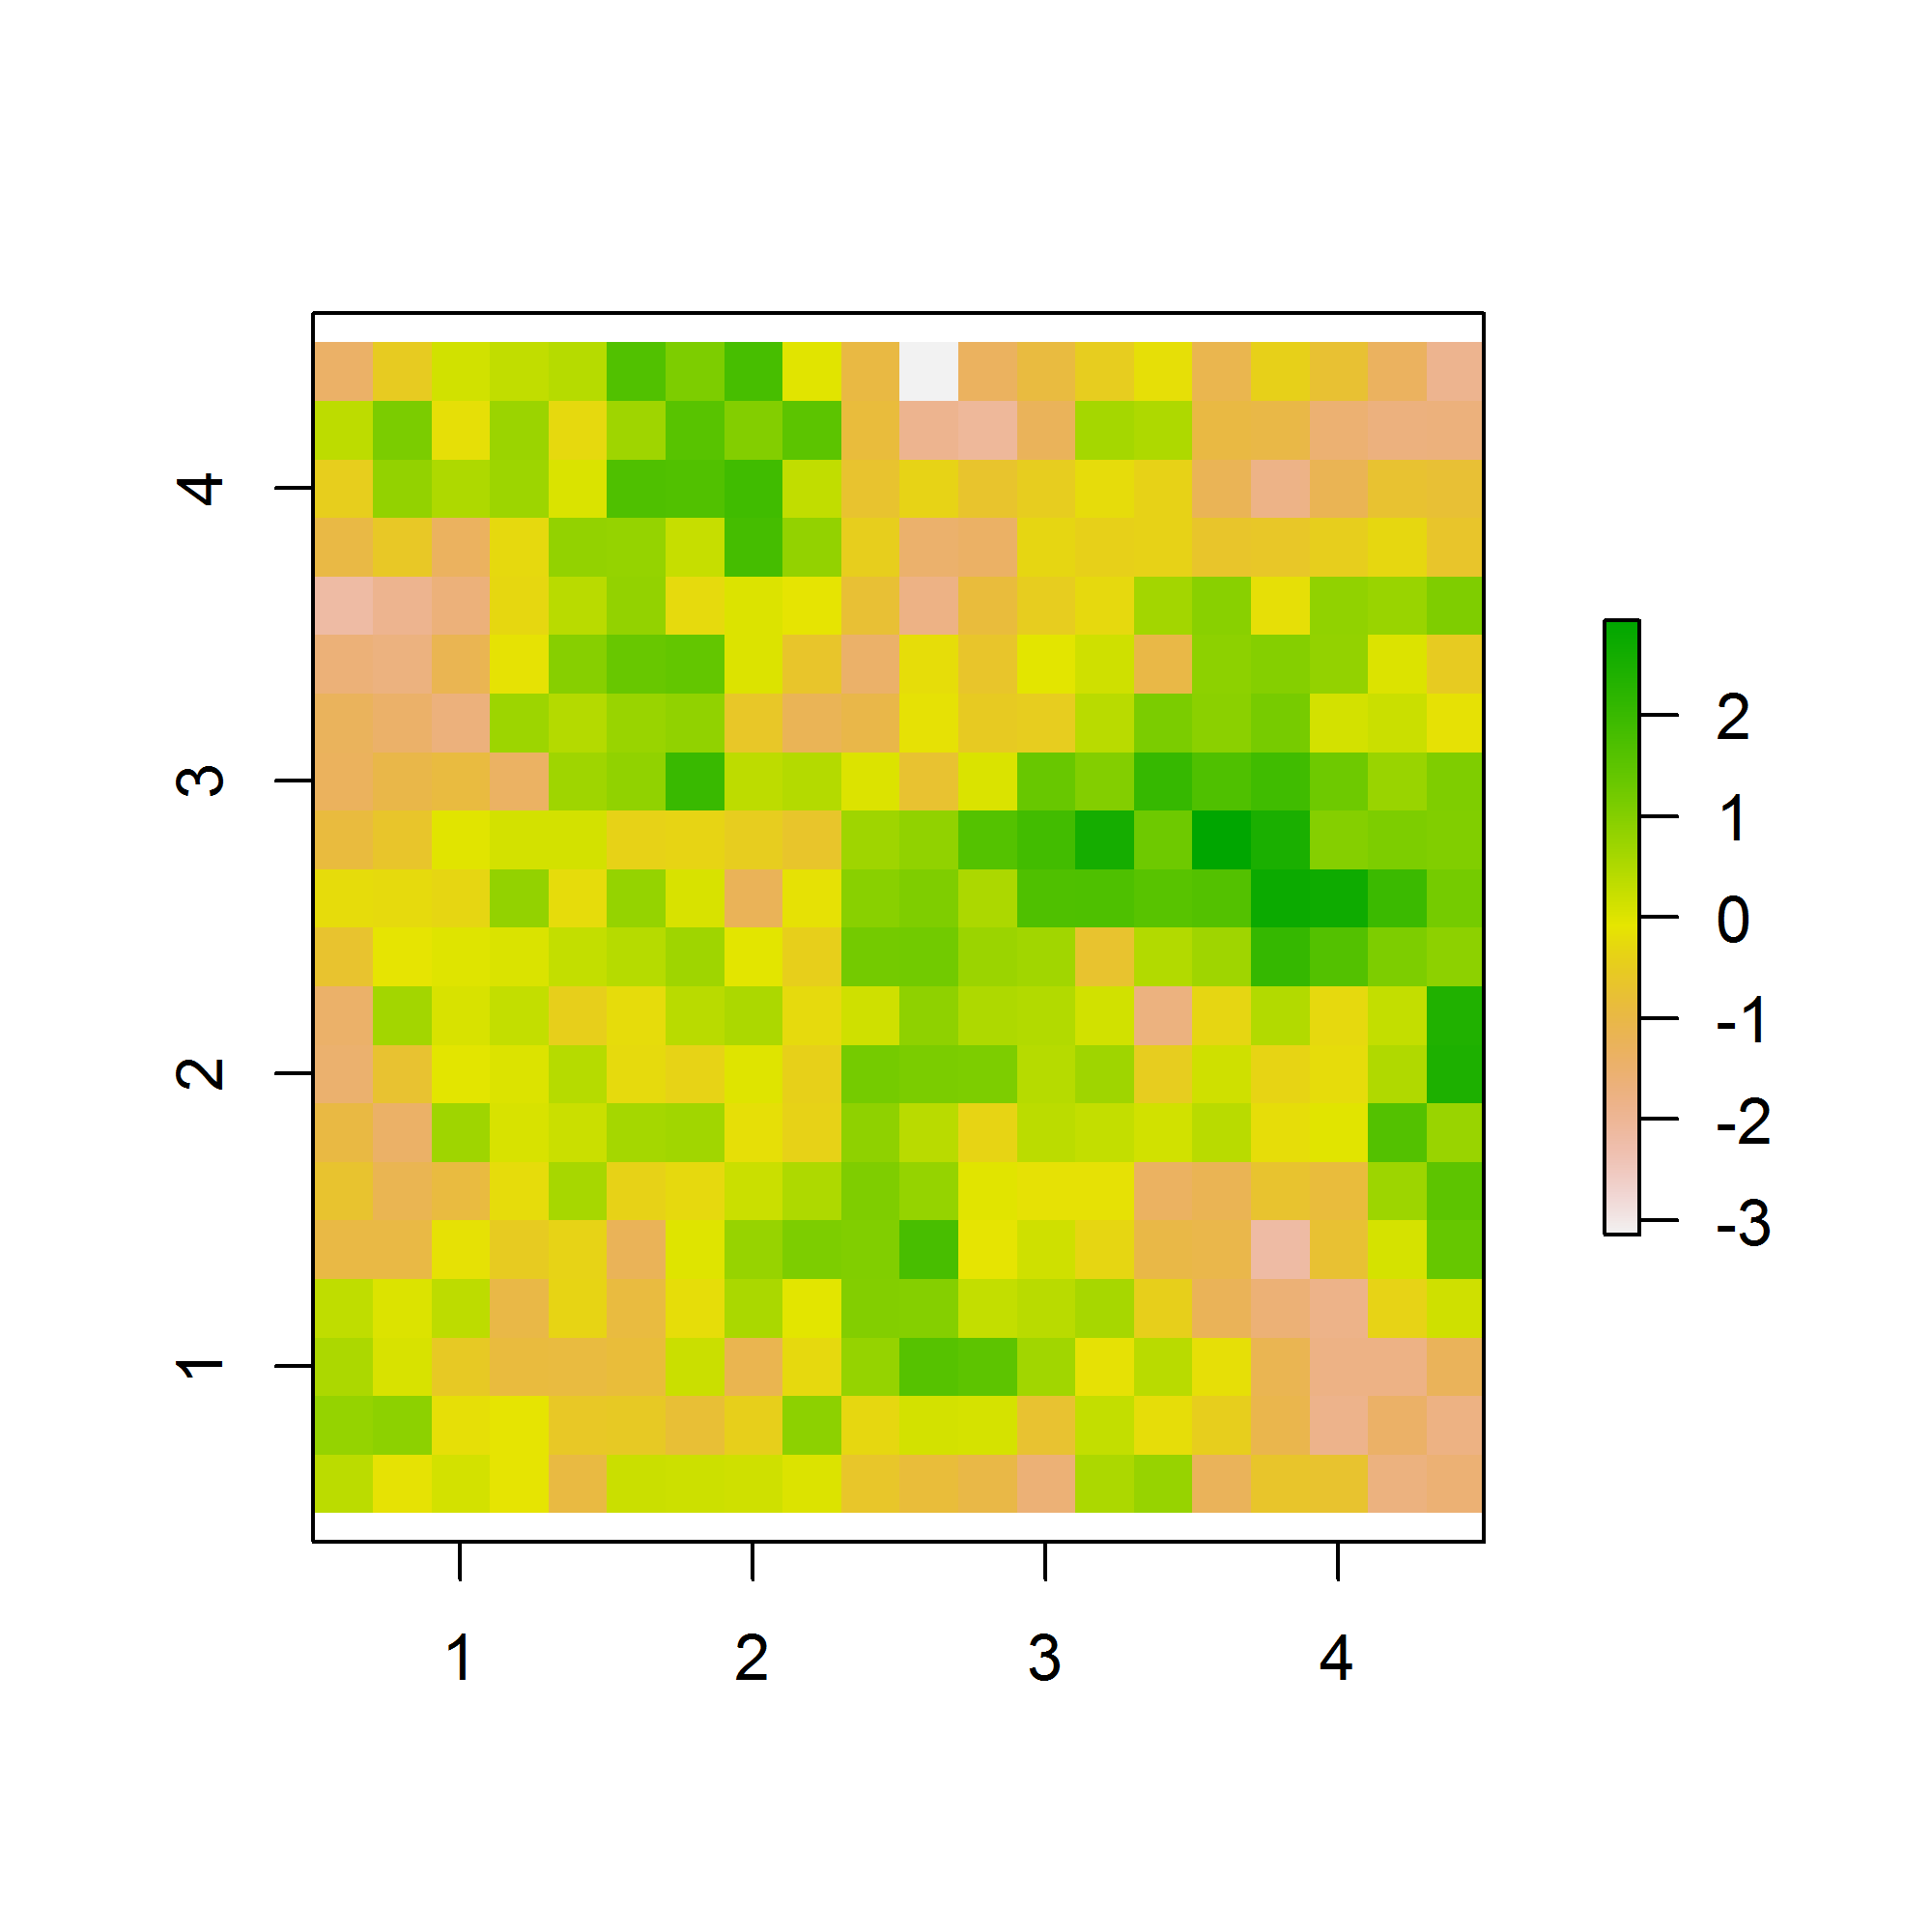
\includegraphics[height=2.5in,width=2.5in]{Ch10-EcolDist/figs/raster_krige} &
\end{tabular}
\caption{Two covariates (defined on a $20 \times 20$ grid) used in simulations.
 Left panel shows a 
 covariate with systematic structure meant 
to mimic distance from some feature, and the right panel
 shows a ``patchy'' covariate. 
A hypothetical
  realization of $N=100$ activity centers (blue dots) is superimposed
  on the left figure,
along with 16 trap locations. }
\label{ecoldist.fig.raster100}
\end{figure}


When distance is defined by the cost-weighted distance metric given
by Eq. \ref{eq.lcp} then individual space-usage varies
spatially in response to the landscape covariate(s) used in the
distance metric.  As a consequence, home ranges contours are no longer
circular, as in SCR models based on Euclidean distance.
 For example, using one of the covariates we use in
our simulation study below (Fig. \ref{ecoldist.fig.raster100}, right
panel) with a Gaussian pdf detection function but having distance
metric defined by Eq. \ref{eq.lcp}, produces home ranges such
as those shown in Fig. \ref{fig.homeranges}. 


\begin{figure}
\begin{center}
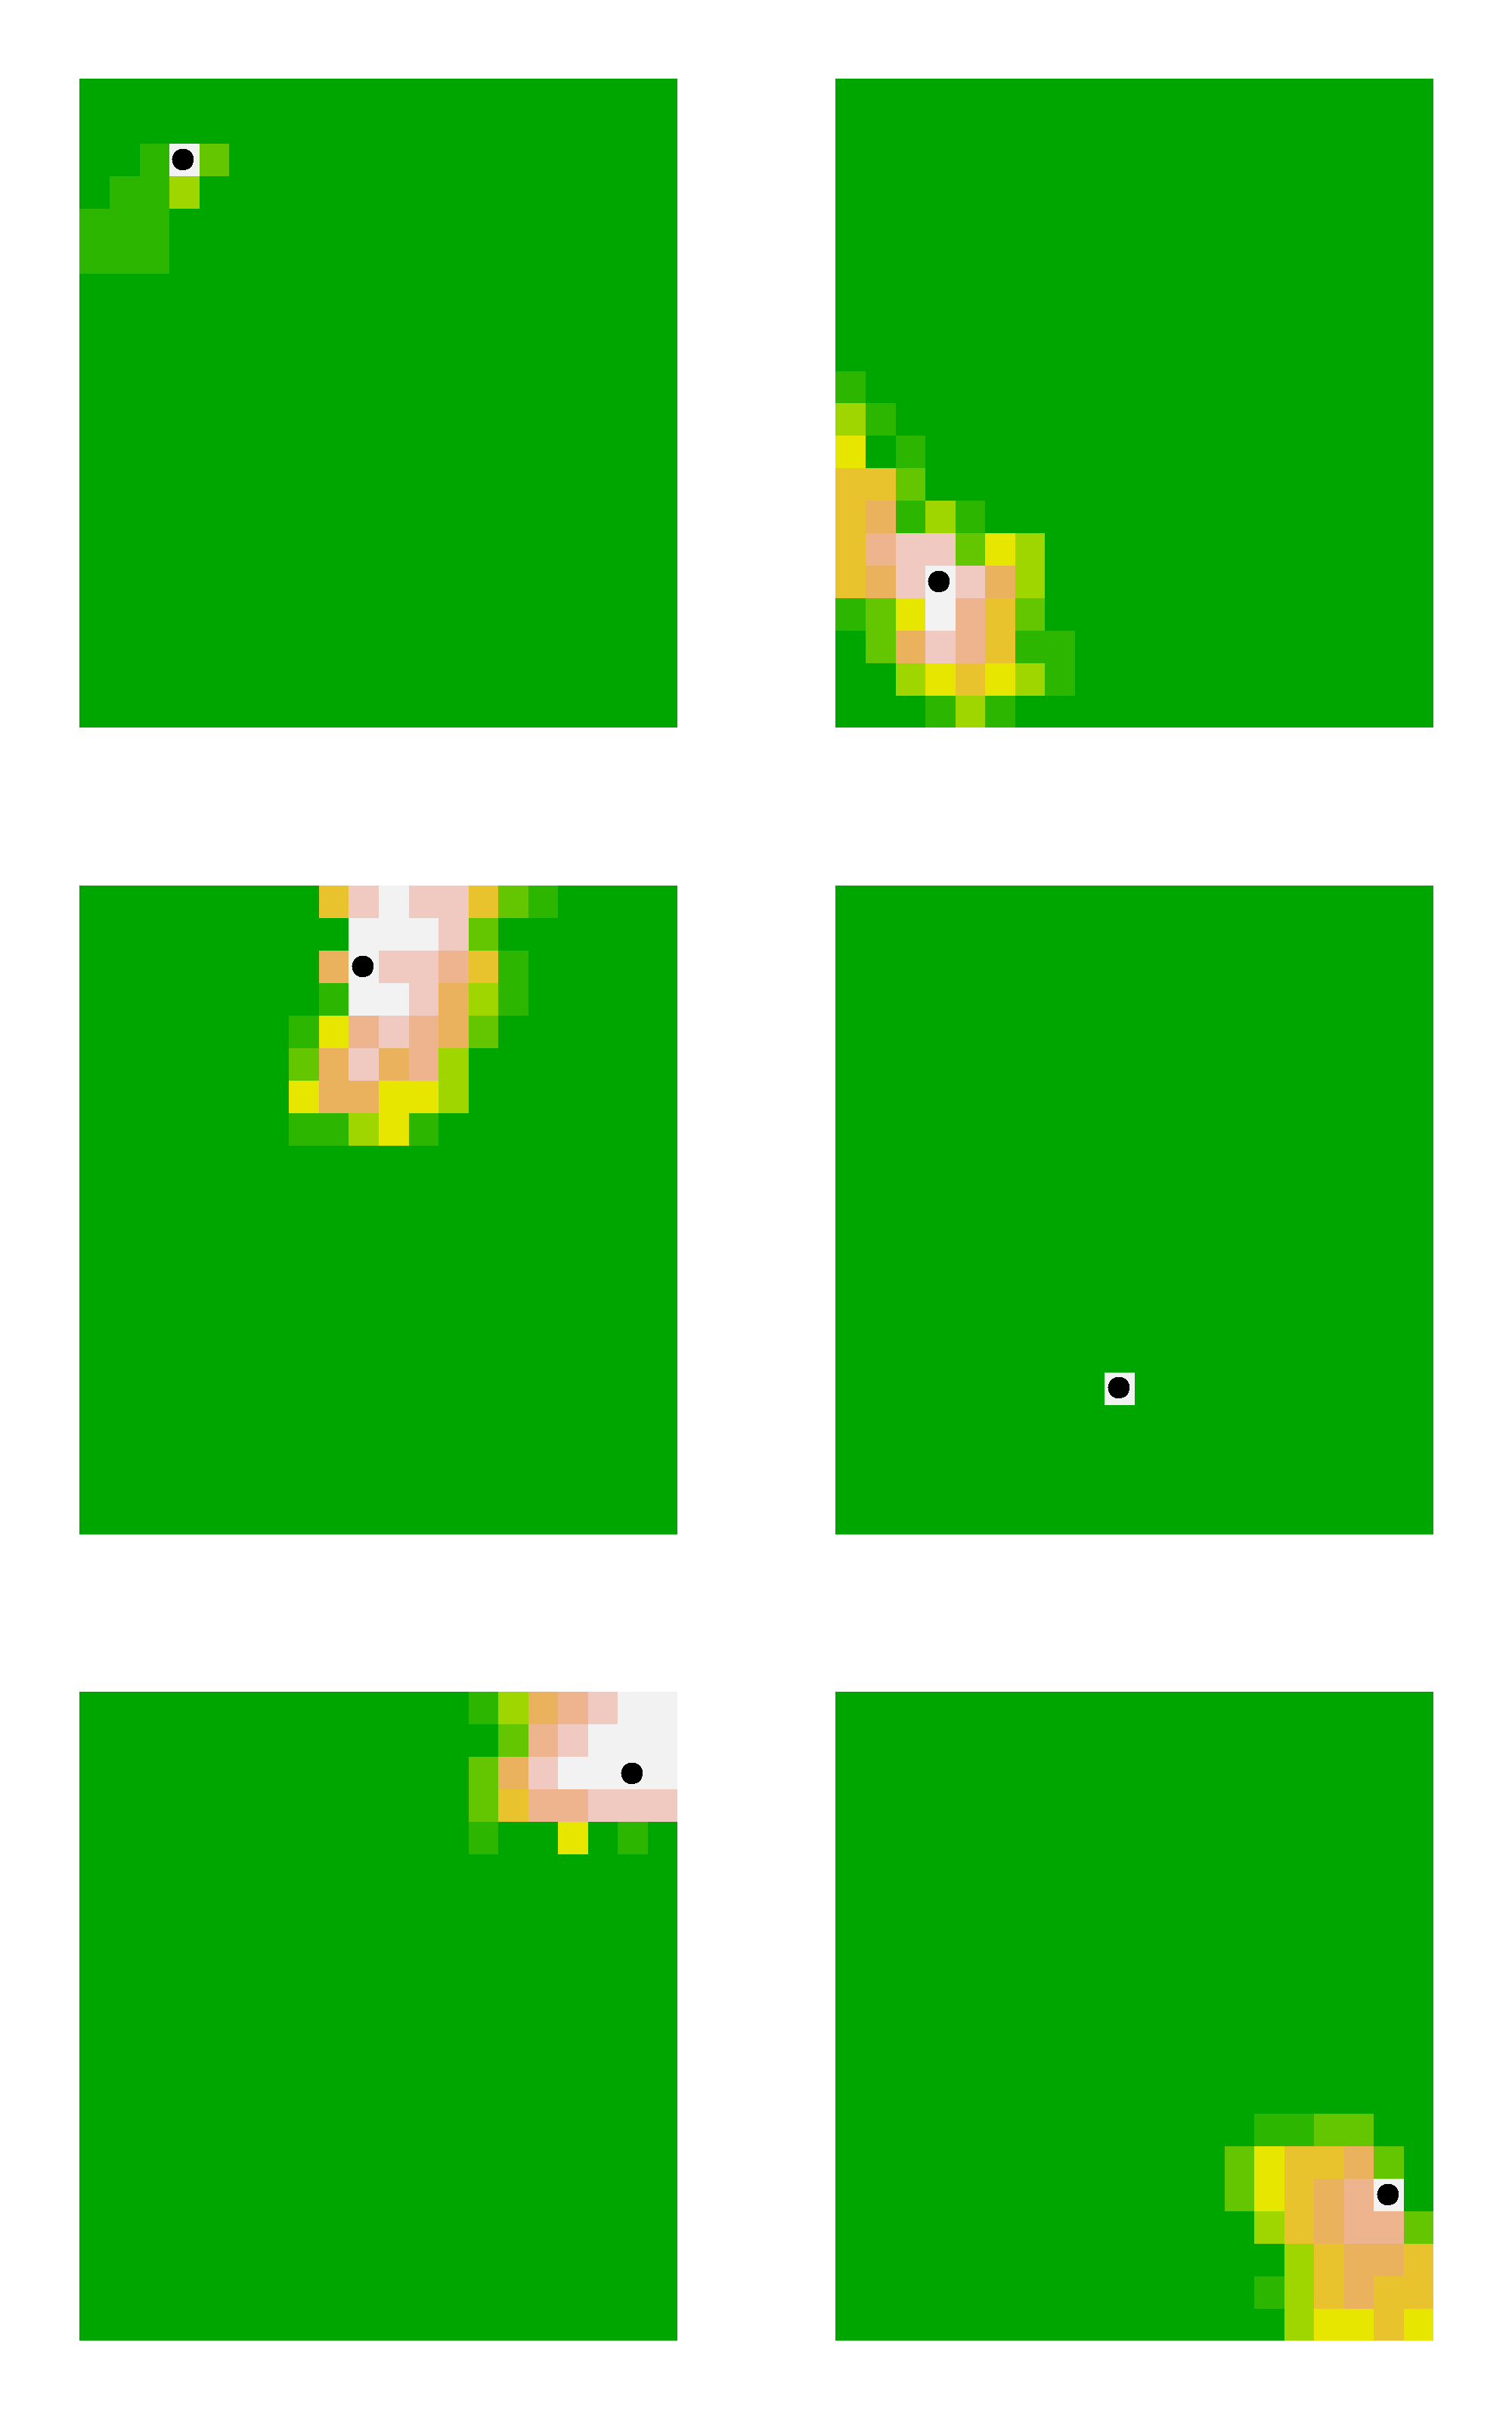
\includegraphics[height=6in,width=3.75in]{Ch10-EcolDist/figs/home_ranges}
\end{center}
\caption{
Typical home ranges for 6 individuals based on the cost surface shown in the right panel of 
  Fig. \ref{ecoldist.fig.raster100} with $\alpha_{2}=1$. The black dot indicates the home
  range center and the pixels around each home range center are shaded
according to the probability of encounter, if a trap were located in
that pixel.
}
\label{fig.homeranges}
\end{figure}

To simulate data, 
 we have to load the \mbox{\tt
scrbook} package and call the function \mbox{\tt make.EDcovariates} to generate
our raster covariates (see the help file for how that is done). We
process the covariate into a least-cost path distance
matrix, and then simulate observed encounter data using standard methods
which we have used many times previously in this book. The complete set
of {\bf R} commands is:
{\small
\begin{verbatim}
### Grab a covariate
library("scrbook")
out<-make.EDcovariates()
covariate<-out$covariate.patchy
set.seed(2013)

### prescribe some settings
N<-200
alpha0<- -2
sigma<- .5
alpha1<- 1/(2*sigma*sigma)
alpha2<-1
K<- 5
S<-cbind(runif(N,.5,4.5),runif(N,.5,4.5))

# make up some trap locations
xg<-seq(1,4,1); yg<-4:1
traplocs<-cbind( sort(rep(xg,4)),rep(yg,4))
points(traplocs,pch=20,col="red")
ntraps<-nrow(traplocs)

### make a raster and fill it up with the "cost"
r<-raster(nrows=20,ncols=20)
projection(r)<- "+proj=utm +zone=12 +datum=WGS84"
extent(r)<-c(.5,4.5,.5,4.5)
cost<- exp(alpha2*covariate)
### compute 
tr1<-transition(cost,transitionFunction=function(x) 1/mean(x),directions=8)
tr1CorrC<-geoCorrection(tr1,type="c",multpl=FALSE,scl=FALSE)
D<-costDistance(tr1CorrC,S,traplocs)
probcap<-plogis(alpha0)*exp(-alpha1*D*D)

# now generate the encounters of every individual in every trap
Y<-matrix(NA,nrow=N,ncol=ntraps)
for(i in 1:nrow(Y)){
 Y[i,]<-rbinom(ntraps,K,probcap[i,])
}
Y<-Y[apply(Y,1,sum)>0,]
\end{verbatim}
}










\section{Likelihood Analysis of Ecological Distance Models}
\label{ecoldist.sec.mle}

Throughout much of this book we rely on Bayesian analysis by MCMC
mostly using {\bf BUGS}, but sometimes (as in Chapt. \ref{chapt.mcmc})
developing our own implementations. However, occasionally we prefer to
use likelihood estimation, such as when we can compare a set of models
directly by likelihood either to do a direct hypothesis test of a
parameter, or to tabulate a bunch of AIC values. For
the class of models that use least-cost path, we also 
prefer likelihood methods not because they have any
conceptual or methodological benefit, but simply because they are more
computationally efficient to implement \citep{royle_etal:2012ecol}.

There are no technical considerations in adapting our
 formulation of maximum likelihood estimation
\citep{borchers_efford:2008} from Chapt. \ref{chapt.mle} for the class
of models based on least-cost path. This is really just a
straightforward adaptation in which we replace the Euclidean distance
with least-cost path.
Consider the Bernoulli model in which 
the individual- and trap-specific observations have a binomial
distribution conditional on the latent variable ${\bf s}_{i}$:
\begin{equation}
  y_{ij}| {\bf s}_{i} \sim \mbox{Binomial}(K, p_{\bm \alpha}(d_{lcp}({\bf x}_{j},{\bf s}_{i};\alpha_{2}); \alpha_{0}, \alpha_{1})
\label{ecoldist.eq.cond-on-s}
\end{equation}
where we have indicated the dependence of $p$ on the parameters
${\bm \alpha} =(\alpha_{0},\alpha_{1},\alpha_{2})$, and also $d_{lcp}$ which
itself depends on $\alpha_{2}$, and the latent variable ${\bf s}$.
We note that the only difference between likelihood analysis of this
model and the standard Bernoulli model, is the use of $d_{lcp}$ here. 
For the random effect we have ${\bf s}_{i} \sim  \mbox{Uniform}({\cal
  S})$, we can easily compute the integrated likelihood.

We have an R script in the \mbox{\tt scrbook} package?
adapated from Royle et al. ....

We provide an {\bf R} function to evaluate the likelihood, and
optimize it 
using the {\bf R} function \mbox{\tt nlm}.
The likelihood is given in the {\tt scrbook} package as the function
\mbox{\tt intlik3ed}. The help file
provides an example of its usage and for simulating data.
To use this function the cost covariate $z({\bf x})$ has to be of class
\mbox{\tt RasterLayer} which requires packages \mbox{\tt sp} and
\mbox{\tt raster} to manipulate.
%The following is a stylized and more concise version of the actual
%function, and 
%We apply this in the following section.

\begin{comment}
{\small
\begin{verbatim} 

$I would try to make this as readable as possible by doing four things:
- add hashed-out comments
- put stuff in paragraphs
- add a few spaces before lines inside if statements and for loops
- clean up code as much as possible
$
intlik3ed<-function(start=NULL,y=y,K=NULL,X=traplocs,
distmet="ecol",covariate,alpha2=NA){

nc<-covariate@ncols
nr<-covariate@nrows
Xl<-covariate@extent@xmin
Xu<-covariate@extent@xmax
Yl<-covariate@extent@ymin
Yu<-covariate@extent@ymax
### ASSUMES SQUARE RASTER -- NEED TO GENERALIZE THIS
delta<- (Xu-Xl)/nc
xg<-seq(Xl+delta/2,Xu-delta/2,delta)
yg<-seq(Yl+delta/2,Yu-delta/2,delta)
npix.x<-length(xg)
npix.y<-length(yg)
area<- (Xu-Xl)*(Yu-Yl)/((npix.x)*(npix.y))
G<-cbind(rep(xg,npix.y),sort(rep(yg,npix.x)))
nG<-nrow(G)

if(distmet=="euclid")
D<- e2dist(X,G)

if(distmet=="ecol"){
if(is.na(alpha2))
alpha2<-exp(start[4])
cost<- exp(alpha2*covariate)
tr1<-transition(cost,transitionFunction=function(x) 1/mean(x),directions=8)
tr1CorrC<-geoCorrection(tr1,type="c",multpl=FALSE,scl=FALSE)
D<-costDistance(tr1CorrC,X,G)
}

alpha0<-start[1]; alpha1<-start[2]; n0<-exp(start[3])

probcap<- (exp(alpha0)/(1+exp(alpha0)))*exp(-alpha1*D*D)
Pm<-matrix(NA,nrow=nrow(probcap),ncol=ncol(probcap))
ymat<-y ; ymat<-rbind(y,rep(0,ncol(y)))
lik.marg<-rep(NA,nrow(ymat))
for(i in 1:nrow(ymat)){
Pm[1:length(Pm)]<- (dbinom(rep(ymat[i,],nG),rep(K,nG),probcap[1:length(Pm)],log=TRUE))
lik.cond<- exp(colSums(Pm))
lik.marg[i]<- sum( lik.cond*(1/nG) )
}
nv<-c(rep(1,length(lik.marg)-1),n0)
part1<- lgamma(nrow(y)+n0+1) - lgamma(n0+1)
part2<- sum(nv*log(lik.marg))
out<-  -1*(part1+ part2)
out
}
\end{verbatim}
}
\end{comment}


\subsection{Example of SCR with Least-Cost Path}

Now we use the {\bf R} function \mbox{\tt nlm} along with
our \mbox{\tt intlik3ed} function to  obtain the MLEs of the
model parameters for the data simulated 
in sec. \ref{ecoldist.sec.simulating}.
 We'll do that for both the standard Euclidean distance
and then for the ecological distance based on the ``patchy''
covariate using the following commands:
{\small
 \begin{verbatim}
frog1<-nlm(intlik3ed,c(alpha0,alpha1,3)),hessian=TRUE,y=Y,K=K,X=traplocs,
               distmet="euclid",covariate=covariate,alpha2=1)

frog2<-nlm(intlik3ed,c(alpha0,alpha1,3,-.3),hessian=TRUE,y=Y,K=K,X=traplocs,
               distmet="ecol",covariate=covariate,alpha2=NA)
\end{verbatim}
}
The abbreviated output for the two model fits
\begin{verbatim}
> frog1

$minimum
[1] 133.4951

$estimate
[1] -1.885005  1.247305  3.549064

[... deleted ....]


> frog2
$minimum
[1] 70.11916

$estimate
[1] -1.78029983  2.47083431  4.45867628  0.04560194

[... deleted ...]
\end{verbatim}

{\bf XXXX Insert Table XXXXX remove some results XXXXX}
Table:
           a0      a1    a2    log(n0)  Nhat   AIC
 truth
 SCR
 SCR/LP
{\bf XXXX Insert Table XXXXX}

The model based on least-cost path (the data generating model) appears
to be much preferred in terms of negative log-likelihood.
The output parameter order is $(\alpha_{0}, \alpha_{1}, log(n_{0}), and
log(\alpha_{2}))$ (remember, we want to keep $\alpha_{2}$
positive, so it's logarithm is estimated). 
The data generating parameter values were
$\alpha_{0} = - 2$, 
$\alpha_{1} = 2$ and $log(\alpha_{2}) = 0$.
The simulated sampling produced a sample of 96 individuals and so
$n_{0} = 104$, so $log(n_{0}) = 4.64$. We see that the 
 MLEs of the least-cost path model are pretty close whereas they are
 not so close under the misspecified model based on Euclidean distance.






\section{Bayesian Analysis}

While implementation of these ecological distance SCR models is
reasonably straightforward, we do not believe the model can be fitted
in the  {\bf BUGS} engines because least-cost path distance cannot be computed.
It would be possible to fit the models
in {\bf BUGS} if the parameter $\alpha_{2}$ was fixed. In that case,
one could compute the distance matrix ahead of time and reference the
required elements for a given ${\bf s}$.
Alternatively, it would be possible to write a custom MCMC routine
using the methods we present in Chapt. \ref{chapt.mcmc}, although we
have not yet developed our own MCMC implementation of SCR models with
ecological distance metrics. 


\section{Simulation Evaluation of the MLE}

\citet{royle_etal:2012ecol}
carried-out a limited simulation study to evaluate the
general statistical performance of the density estimator under
this new model, the effect of mis-specifying the model with a
normal Euclidean distance metric and evaluate the general bias and
precision properties of the MLE.
We recapitulate their results here.
For population sizes of 100 and 200, individuals with activity
centers randomly distributed on the $20 \times 20$ landscape, they
subjected individuals
to encounter by 16 traps arranged in a $4\times 4$ grid
using a Gaussian
encounter model with least-cost path distance metric:
\[
log(p_{ij})= \alpha_{0} + \alpha_{1} d_{lcp}({\bf x}_{j},{\bf
  s}_{i}; \alpha_{2})^{2}
\]
where  $\alpha_{0} = -2$ and $\alpha_{1} = 2$, the latter value
corresponding to $\sigma = 0.5$ of a stationary bivariate normal home
range model.  Different numbers of replicate samples were considered,
$K=3,5,10$
(e.g., nights in a camera trapping study), in order
to produce varying sample
sizes.
For each of the ``systematic'' and ``patchy'' landscapes defined
previously, 200 data sets were simulated and, for each of those, two
different models were fitted: the misspecified Euclidean distance
model; and (ii) the true data-generating model but estimating the
relative cost parameter by maximum likelihood.

\subsection{Simulation Results}

For both landscapes and all simulation conditions (levels of $K$ and
$N$) the average sample sizes of individuals captured are given in
Tab. \ref{tab.samplesize}.  
\begin{table}[h]
\centering
\caption{
Expected sample sizes of captured individuals under each configuration of
$N$ (population size for the prescribed state-space) and $K$ (number of replicate samples).
}
\begin{tabular}{l|rrrr}
 & \multicolumn{2}{c}{Systematic} & \multicolumn{2}{c}{Patchy}  \\
    & N=100 &  N=200  &   N=100 &  N=200  \\ \hline
K=3 &  38.69 &   78.17  &   37.30 &   74.93  \\
K=5 &  51.10 &  103.18  &   51.89 &  103.71 \\
K=10&  65.81 &  132.39  &   69.44 &  138.76 \\
\end{tabular}
\label{tab.samplesize}
\end{table}
The simulation results for estimating $N$
for the prescribed state-space are presented in Tab.
\ref{tab.results1}.  For the ``patchy'' landscape we see extreme
bias in estimates of $N$ when the Euclidean distance is used. There is
moderate small sample bias of 3-5\% in the MLE of $N$ using the
least-cost distance which becomes negligible as $K$ increases. For
$N=200$ the bias is on the order of 2\% for the lowest sample size
case ($K=3$) but negligible otherwise.  Interestingly, for the
landscape exhibiting systematic structure, there is a persistent bias
in the MLE of $N$ of 1-3\% even for the highest level of $K$.
As noted by \citet{royle_etal:2012ecol}, 
this is due to the fact that
the state-space is small relative to the extent of the trapping grid and
sensitivity to a state-space that is too small is expected because the
support of the integrand is truncated. In the particular case of the
systematic landscape, we find that, in the NW corner of the raster
where cost of movement is low, individuals use large areas of space,
and the fitted model is under-stating the apparent
heterogeneity in encounter probability for the prescribed raster.  \citet{royle_etal:2012ecol}
found that the issue is resolved when the traps are moved away from
the boundary (results shown in Tab. \ref{tab.results3}).

The performance of estimating the cost parameter $\alpha_{2}$ mirrors
the results for estimating $N$ for the prescribed state space. In the
patchy landscape where we don't expect a systematic gradient in space
usage around the edge of the state-space, we see
(Table \ref{tab.results2}) that $\alpha_{2}$ is estimated with
diminishing bias as the sample size increases, but with persistent
bias due to truncation of the likelihood under the systematic
landscape which, as with the MLE of $N$, is resolved by moving the
traps away from the edge of the raster. Equivalently, in practice,
this could be resolved by expanding the raster away from the trap
locations so that all regions used by animals exposed to capture are
included in the state-space.




\begin{table}[htp]
\label{tab.results1}
{\small
\caption{Simulation results for estimating population size $N$ for a prescribed state-space with
$N=100$ or $N=200$ and various levels of replication ($K$) chosen to affect the observed sample
size of individuals (Tab. \ref{tab.samplesize}). For each simulated
data set, the SCR model was fitted by maximum likelihood with
standard Euclidean distance (``euclid''), or least-cost path 
(``lcp''), which was the true data-generating model.
The summary statistics of the
sampling distribution reported are the mean, standard deviation
(``SD'') and quantiles (0.025, 0.50, 0.975).
}
{\bf Systematic trend raster:} \\
\begin{tabular}{l|rrrrr|rrrrr}
         & \multicolumn{5}{c}{N=100   } & \multicolumn{5}{c}{N=200  }  \\
         &   mean &  SD  & 0.025 & 0.50 & 0.975  & mean  & SD   & 0.025 & 0.50  & 0.975 \\ \hline
K=3      &        &      &       &      &        &       &      &       &       &       \\
euclid   &   63.65& 12.62& 44.77 & 61.17&  90.98 & 126.68& 17.05&  98.93& 124.49& 168.26 \\
lcp      &  101.93& 21.68& 67.95 &101.56& 156.21 & 201.58& 28.14& 154.96& 200.15& 263.20\\
K=5      &        &      &       &      &        &       &      &       &       &        \\
euclid   &  64.60 & 7.11 & 51.52 & 63.86&  77.33 & 130.02& 10.25& 113.48& 128.96& 151.32\\
lcp      &  98.94 &12.97 & 74.68 & 99.00& 123.88 & 198.80& 19.60& 166.87& 197.97& 239.46\\
K=10     &        &      &       &      &        &       &      &       &       &       \\
euclid   &  69.24 & 4.83 & 59.37 & 69.47&  79.18 & 139.83&  7.62& 125.65& 139.65& 154.82\\
lcp      &  97.53 & 8.18 & 82.02 & 97.62& 113.16 & 195.19& 13.28& 171.63& 194.58& 217.96\\ \hline
\end{tabular}
\\
{\bf Patchy ``random'' raster: } \\
\begin{tabular}{l|rrrrrrrrrr}
         & \multicolumn{5}{c}{N=100  } & \multicolumn{5}{c}{N=200   }  \\
         &   mean &  SD  & 0.025 & 0.50  & 0.975  & mean  & SD   & 0.025 & 0.50  & 0.975 \\ \hline
K=3      &        &      &       &       &        &       &      &       &       &       \\
euclid   &  78.68 & 18.12& 49.40 & 76.34 & 125.47 & 154.34& 33.74& 107.00& 146.34& 221.43\\
lcp      & 110.96 & 28.65& 69.55 &106.98 & 181.84 & 208.77& 49.29& 141.68& 197.89& 325.77\\
K=5      &        &      &       &       &        &       &      &       &       &        \\
euclid   &  77.85 & 11.55& 59.17 & 77.44 & 101.14 & 153.39& 15.57& 129.31& 149.54& 185.38\\
lcp      & 104.44 & 15.79& 78.38 &101.47 & 139.55 & 200.91& 20.78& 164.42& 200.47& 246.46\\
K=10     &        &      &       &       &        &       &      &       &       &       \\
euclid   &  78.01 & 5.26 & 68.00 & 77.96 & 87.81  & 156.27&  8.51& 142.17& 156.05& 174.55\\
lcp      & 100.42 & 7.56 & 86.72 &100.34 & 115.47 & 198.45& 11.44& 180.06& 198.04& 219.52\\ \hline
\end{tabular}
}
\end{table}





\begin{table}[htp]
\centering
\caption{
Mean of sampling distribution of the cost function parameter
$\alpha_{2}$ for the different simulation
conditions.
}
\begin{tabular}{l|rrrr}
 & \multicolumn{2}{c}{Patchy} & \multicolumn{2}{c}{Systematic} \\
    & N=100 &  N=200  &   N=100 &  N=200  \\ \hline
$K=3$  &   1.05&    1.03 &     1.17 & 1.14 \\
$K=5$  &   1.02&    1.01 &     1.12 &1.12 \\
$K=10$ &   1.01&    1.00 &     1.10 &1.08 \\
\end{tabular}
\label{tab.results2}
\end{table}




\begin{table}[htp]
{\tiny
\caption{Simulation results for estimating population size $N$ for a prescribed state-space with
$N=100$ or $N=200$ and various levels of replication ($K$) chosen to affect the observed sample
size of individuals. These results correspond to those of the
systematic landscape in Table XXXXXXX  except with the traps
moved 0.5 units in from the boundary of the landscape.
Each grouping of 2 rows (for a given value of $K$) summarizes the
performance of $\hat{N}$ under models based on 
Euclidean distance  (``euclid'') and 
a model based on least-cost path, which was the true data-generating model.
The summary statistics of the
sampling distribution reported are the mean, standard deviation
(``SD'') and quantiles (0.025, 0.50, 0.975).
}
\begin{tabular}{l|rrrrr|rrrrr}
         & \multicolumn{5}{c}{N=100   } & \multicolumn{5}{c}{N=200  }  \\
         &   mean &  SD  & 0.025 & 0.50 & 0.975  & mean  & SD   & 0.025 & 0.50  & 0.975 \\ \hline
K=3      &        &      &       &      &        &       &      &       &       &       \\
euclid   &   84.48& 20.42& 51.16 & 81.51& 140.62 &163.70 &24.55 &126.64 &157.67 &223.63 \\
lcp      &  105.90& 26.19& 65.95 &103.40& 182.30 &201.34 &29.54 &161.88 &192.36 &268.98\\
K=5      &        &      &       &      &        &       &      &       &       &       \\
euclid   & 81.21  &11.33 &61.35  &79.20 & 98.86  &163.27 &13.06 &140.21 &162.97 &185.94\\
lcp      & 100.84 &13.15 &79.96  &99.51 &119.08  &200.25 &16.53 &168.88 &199.29 &227.39\\
K=10     &        &      &       &      &        &       &      &       &       &       \\
euclid   &  80.10 & 7.81 &66.45  &79.14 &93.33   &158.40 & 9.25 &142.74 &157.86 &173.18\\
lcp      & 100.10 & 9.88 &82.31  &100.91&116.27  &197.52 &13.03 &169.49 &200.68 &217.82\\ \hline
\end{tabular}
}
\label{tab.results3}
\end{table}





\section{Distance In an Irregular Patch}
\label{ecoldist.sec.buffer}

We provide another illustration of how to employ ecological distance
calculations in SCR models. This example is meant to mimic 
a situation where we have something like a hard habitat boundary
such as a habitat corridor or park unit or some other block
of relatively homogeneous good-quality habitat for some species. This
particular system (shown in Fig. \ref{ecoldist.fig.corridor}) could
be habitat surrounded by a suburban wasteland of McDonalds and
Wal-Marts, much less hospitable habitat for most species.  For our
purposes, we suppose that individuals live within the buffered
``f-shaped'' 
region, although we could also imagine the negative of the
situation in which individuals live outside of the region, so that the
polygon represents a barrier (a lake) or bad habitat (an urban area)
or similar.  We describe the steps for creating this landscape
shortly, so that you can use a similar process to generate more
relevant landscapes for your own problems.

In this case we're not going to estimate any parameters of the cost
function (though you could adapt the analyses of the previous sections
to do that) but instead we're going to use ecological
distance ideas only to constrain movement within (or to avoid)
landscape features. Note that, normally, distance ``as the crow
flies'' would not be suitable for irregular habitat patches such as
that shown in Fig. \ref{ecoldist.fig.corridor}.  


\subsection{Basic Geographic Analysis in R}

In practical applications our landscape will contain one more more
polygons which delineate good or bad habitat or other important
characterisetics of the landscape.  These might exist as GIS
shapefiles or merely as a text file with coordinates defining polygon
boundaries. To work with polygons in the context of SCR models we need
to create a raster, overlay the polygon and assign values to each pixel
depending on whether pixels are in the polygon or not, or how far they
are from polygon boundaries. These operations are relatively easy to
do within a GIS system but we need to be able to do them in ${\bf R}$
in order to compute the least-cost paths needed in the likelihood
evaluation. Some additional geographic analyses have been discussed in
secs. \ref{ecoldist.sec.shapefile} and \ref{mcmc.sec.state-space}
where we talked about reading in the shapefile and doing SCR calculations
on that. 

Often we will have GIS shapefiles that define polygons but, here, we 
 create a set of polygons by
buffering and joining some line segments.
In the {\bf R} library \mbox{\tt scrbook}, we provide
 a function \mbox{\tt make.seg} which allows you to make such
 lines segments given a
specific trap region.  To involve \mbox{\tt make.seg} we first
create a plot region and then call \mbox{\tt make.seg} which has a
single argument being the number of points used to define the line
segment. The user will click on the visual display until the required
number of points has been obtained by \mbox{\tt make.sec}. 
In the following set of commands we generate two line
segments, \mbox{\tt l1} consisting of 9 points and \mbox{\tt l2}
consisting of 5 points, and these reside in a geographic region
enclosedd by $[0,10] \times [0,10]$:
{\small
\begin{verbatim}
library("scrbook")
library("sp")
plot(NULL,xlim=c(0,10),ylim=c(0,10))
l1<-make.seg(9)
plot(l1)
l2<-make.seg(5)
plot(l1)
lines(l2)
\end{verbatim}
}

We used this function as above to create a habitat corridor compose of
line segments of class
\mbox{\tt SpatialLines} from the {\bf R} package \mbox{\tt sp}. The 
corridor can be loaded from \mbox{\tt scrbook} by typing the command
\mbox{\tt data("fakecorridor")}.
This data list has 2 line files in it (\mbox{\tt l1} and \mbox{\tt l2}) and a
trap locations file (\mbox{\tt traps}).
We use some functions from the {\bf R} packages \mbox{\tt sp} and
\mbox{\tt rgeos} to join and
buffer (by 0.5 units) the two segments. The commands are as follows
and the result is shown in Fig. \ref{ecoldist.fig.corridor}.

{\small
\begin{verbatim}
data("fakecorridor")
library("sp")
library("rgeos")

buffer<- 0.5
par(mfrow=c(1,1))
aa<-gUnion(l1,l2)
plot(gBuffer(aa,width=buffer),xlim=c(0,10),ylim=c(0,10))
pg<-gBuffer(aa,width=buffer)
pg.coords<- pg@polygons[[1]]@Polygons[[1]]@coords

xg<-seq(0,10,,40)
yg<-seq(10,0,,40)

delta<-mean(diff(xg))
pts<- cbind(sort(rep(xg,40)),rep(yg,40))
points(pts,pch=20,cex=.5)

in.pts<-point.in.polygon(pts[,1],pts[,2],pg.coords[,1],pg.coords[,2])
points(pts[in.pts==1,],pch=20,col="red")
\end{verbatim}
}

\begin{figure}[h]
\begin{center}
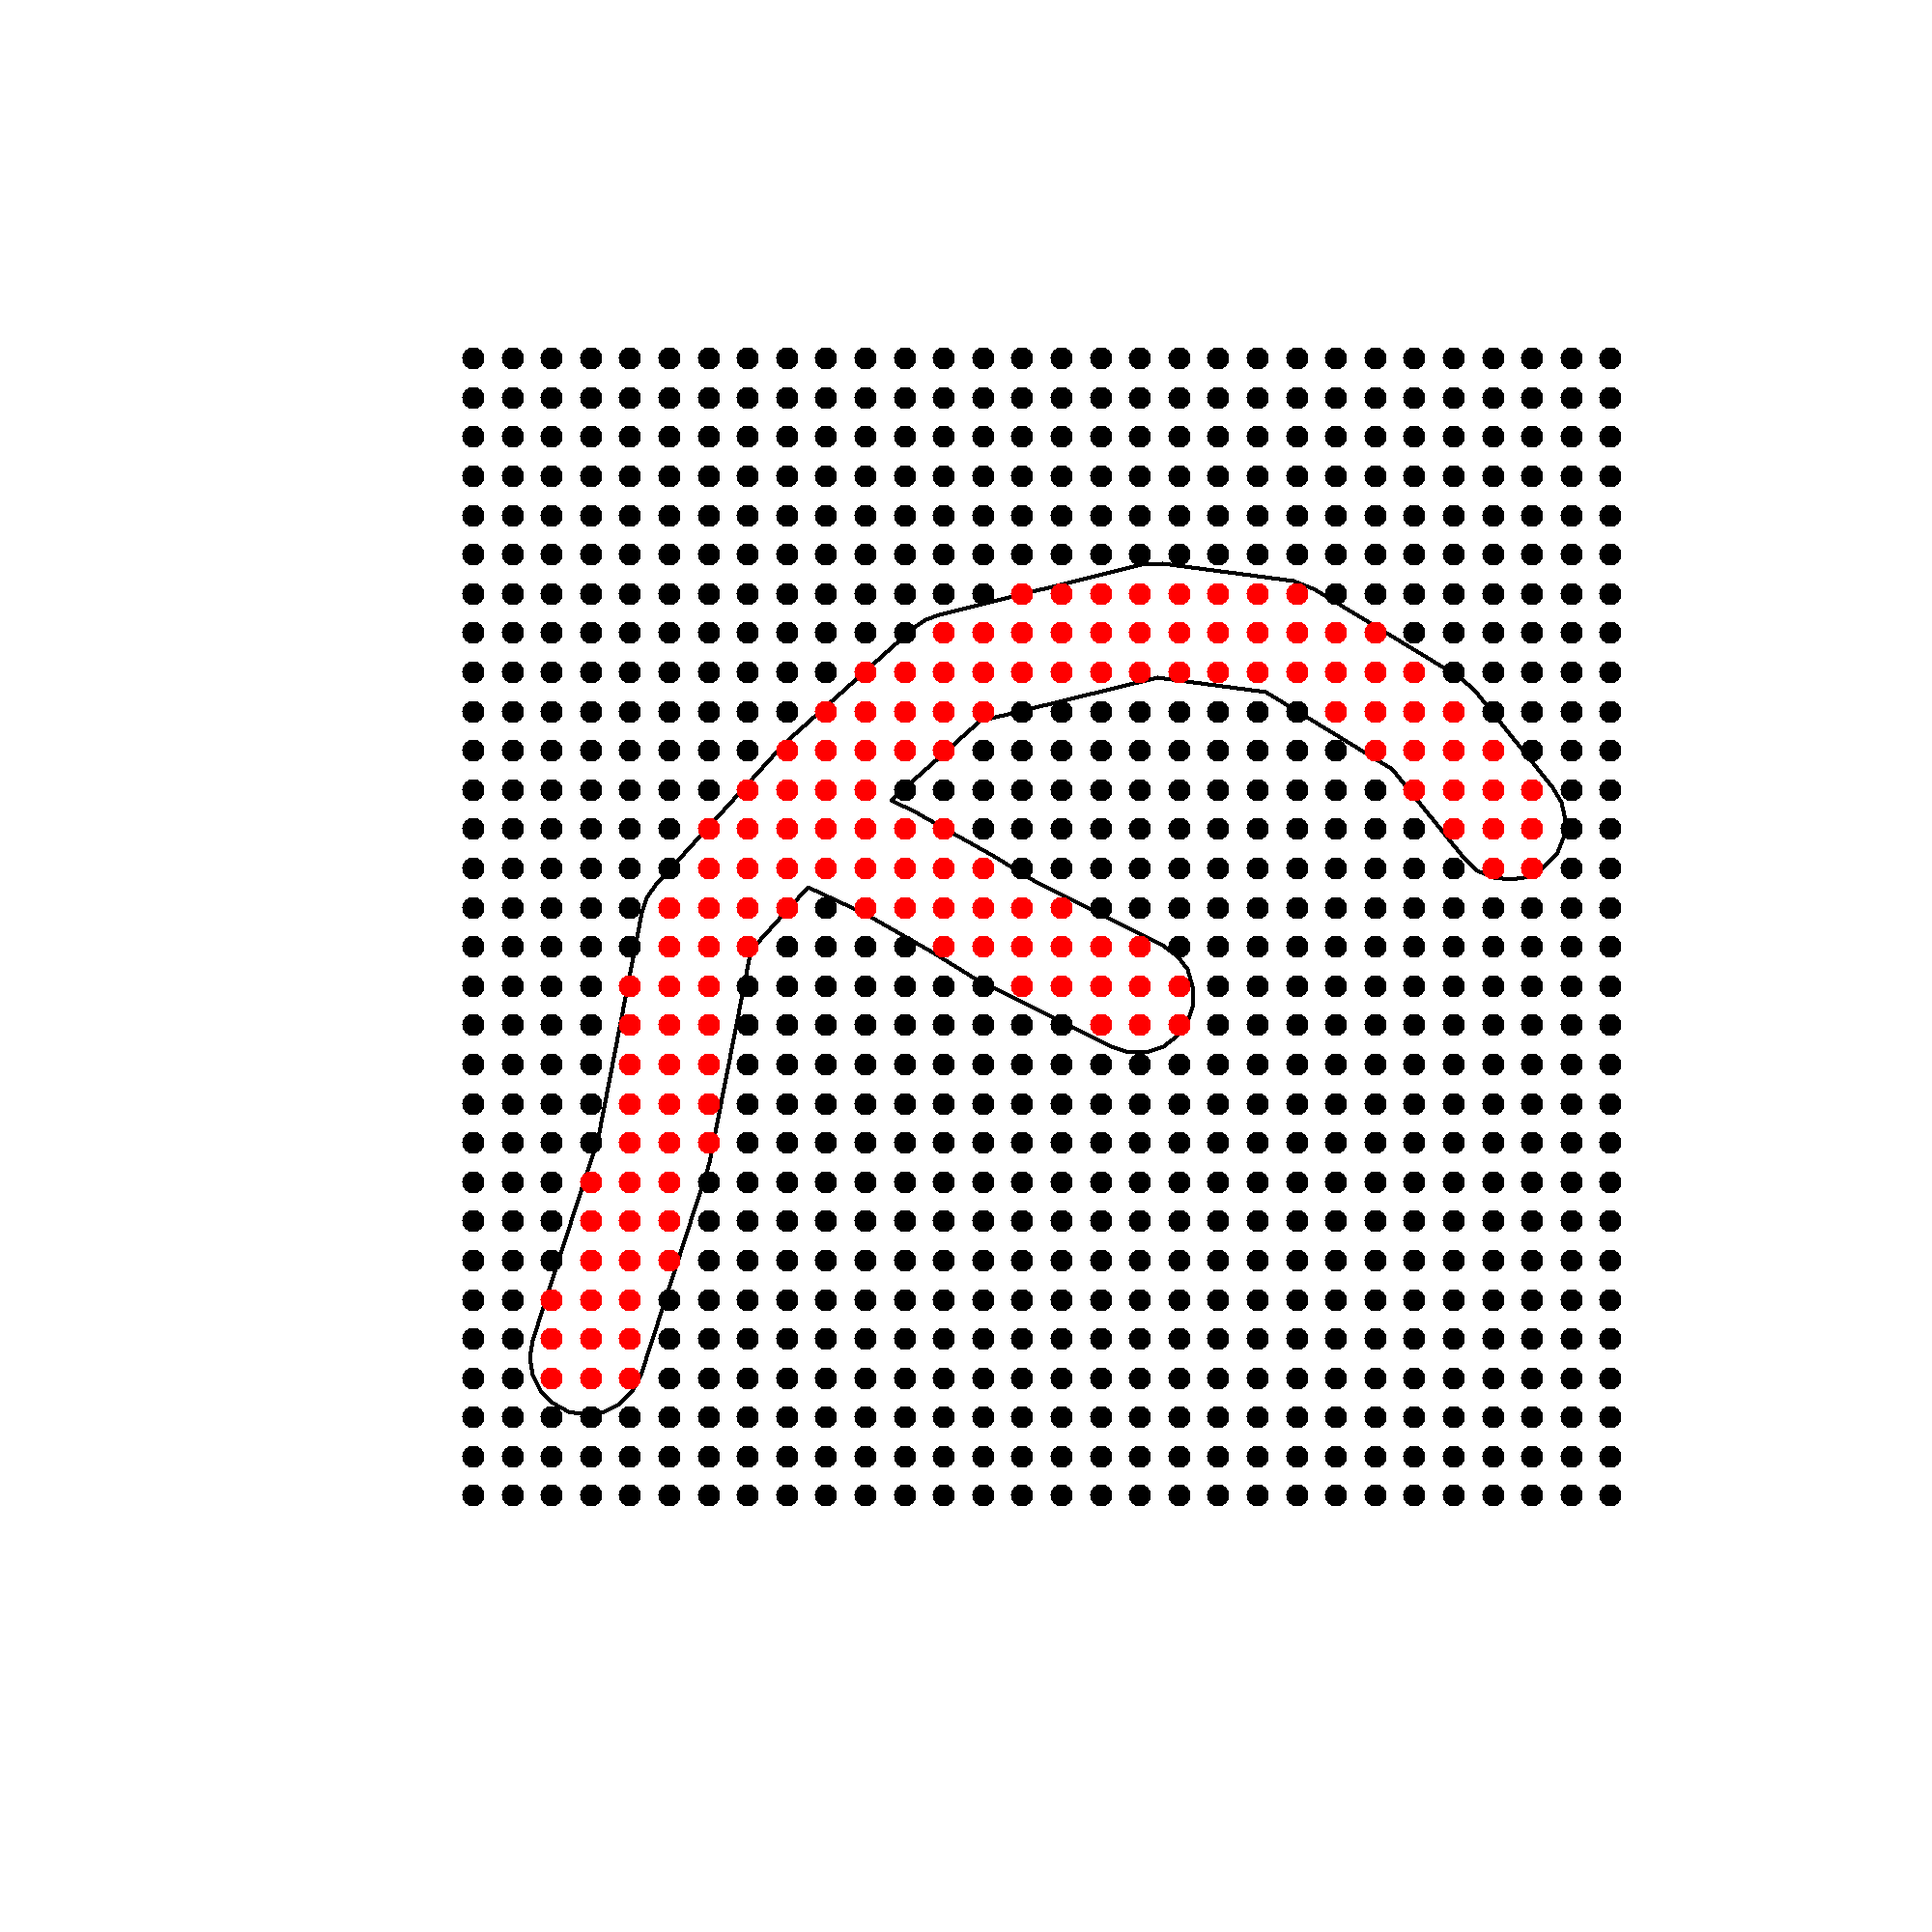
\includegraphics[height=3.25in,width=3.25in]{Ch10-EcolDist/figs/corridor}
\end{center}
\caption{A made-up wildlife corridor or reserve. The boundary outlines
  a polygon of suitable habitat surrounded by suburban development.}
\label{ecoldist.fig.corridor}
\end{figure}


We focus on devising a SCR model for this corridor system and we
imagine that animals will tend to severely avoid leaving the buffered
habitat zone. Therefore, we assign $\mbox{\tt cost}=1$ if a pixel
is within the buffer,
and $\mbox{\tt cost} = 10000$ if a pixel is outside of a
buffer. Therefore the cost to move to a neighboring pixel outside of
the buffered area is $5000.5$ compared to the cost of 1 to move to a
neighboring pixel inside the buffer.

In this example, we're not going to estimate parameters of the cost
function. Therefore, we can compute the least-cost path 
distance matrix one time and modify our likelihood code to accept the
distance matrix as input. We give that likelihood in the library
\mbox{\tt scrbook} as the function \mbox{\tt intlik3edv2}.
We note also that it provides a vector of 0's and 1's that
define any potential state-space restrictions. i.e., 1 if the pixel is
an element of the state-space and 0 if it is not, and so additional
modifications to the geometry of the region could be made.
However, in the analysis of this
simulated data set, we define the state-space to be the buffered
corridor system. 
Here we simulate a population of $N=200$ individuals in the corridor system and so we
restrict our state-space accordingly for purposes of fitting the
model. However we encourage you to refit the model without the
state-space restriction (for fitting the model only) and then
compare the results.  The code for doing all of this is
in the help file for \mbox{\tt intlik3edv2}, which contains the
likelihood function and sample {\bf R} script (\mbox{\tt ?intlik3edv2}). 

{\small
\begin{verbatim}
XXXX NOT SURE HOW MUCH OF THIS TO PUT IN OR NOT XXXXXX
XXXX in any case, it needs reorganized xxxx
xxx
add as many comments as you possibly can without overloading the thing
xxxxx
cost<-rep(NA,nrow(pts))
cost[in.pts==1]<-1      # low cost to move among pixels but not 0
cost[in.pts!=1]<-10000  # high cost

library("raster")
r<-raster(nrows=40,ncols=40)
projection(r)<- "+proj=utm +zone=12 +datum=WGS84"
extent(r)<-c(0-delta/2,10+delta/2,0-delta/2,10+delta/2)
values(r)<-matrix(cost,40,40,byrow=FALSE)
par(mfrow=c(1,1))
plot(r)
points(pts,pch=20,cex=.4)

library("gdistance")
tr1<-transition(r,transitionFunction=function(x) 1/mean(x),directions=8)
tr1CorrC<-geoCorrection(tr1,type="c",multpl=FALSE,scl=FALSE)
costs1<-costDistance(tr1CorrC,pts)
outD<-as.matrix(costs1)
plot(pts,pch=".")
points(pts[in.pts==1,],pch=20,col="red")

library(``scrbook'')
traplocs<-traps$loc
trap.id<-traps$locid
ntraps<-nrow(traplocs)

set.seed(2013)
N<-200
S.possible<- (1:nrow(pts))[in.pts==1]
S.id<-sample(S.possible,N,replace=TRUE)
S<- pts[S.id,]

D<- outD[S.id,trap.id]
eD<- e2dist(S,traplocs)
Dtraps<-outD[trap.id,]

alpha0<- -1.5
sigma<- 1.5
beta<- 1/(2*sigma*sigma)
K<-10

probcap<-plogis(alpha0)*exp(-beta*D*D)
Y<-matrix(NA,nrow=N,ncol=ntraps)
for(i in 1:nrow(Y)){
 Y[i,]<-rbinom(ntraps,K,probcap[i,])
}
Y<-Y[apply(Y,1,sum)>0,]

frog1<-nlm(intlik3edv2,c(-2.5,2,log(4)),hessian=TRUE,y=Y,K=K,X=traplocs,
            S=pts,D=Dtraps,inpoly=in.pts)
frog2<-nlm(intlik3edv2,c(-2.5,2,log(4)),hessian=TRUE,y=Y,K=K,X=traplocs,
            S=pts,D=Deuclid,inpoly=in.pts)
\end{verbatim}
}
This analysis produces the following abbreviated output: 
\begin{verbatim}
> frog1
$minimum
[1] -21.89208

$estimate
[1] -1.3380122  0.3321878  4.3530026

[... deleted ...]

> frog2
$minimum
[1] -21.12804

$estimate
[1] -1.3071132  0.3821317  4.2116319

[... deleted ...]
\end{verbatim}


We find little difference between the two sets of results. In
particular, 150 individuals were captured and so $log(n_{0}) = 3.9$,
and so the correct model produces only a slightly better estimate, and
it is favored by only .7 negative log-likelihood units.
Therefore, for this single instance, the results are not too different.
This is primarily because 
 the distance between individuals, and traps that they are likely
to be captured in, is well-approximated by the Euclidean distance.



\begin{comment}
\section{A stream network}

Later we might add a 3rd prototype situation involving a stream network.

We could use ``distance from stream'' to model effects of habitat
and corridors or whatever
\end{comment}


\section{Summary and Outlook}


All published applications of SCR models to date have been based on models for the
encounter probability that are functions of the 
Euclidean
distance between individual activity centers
 and traps. The obvious limitations are
that it is unaffected by landscape or habitat structure and implies
stationary, isotropic and symmetrical home ranges. These are standard
criticisms of the basic SCR model as universally applied in
practice so far. However, it is not a relevant criticism of the basic
conceptual formulation of SCR models, because, as we have
demonstrated, one can modify the Euclidean distance metric to
accommodate more realistic space usage considerations.  Following
\citet{royle_etal:2012ecol},
we demonstrated how to use
minimum cost-weighted distance (i.e., ``least-cost
path'') between points, and where ``cost'' is characterized by one or
more spatially explicit covariates that are believed to influence
movement or space-usage of individuals.

How animals use space and therefore how distance to a trap is
perceived by individuals is not something that can ever be known. We
can only ever conjure up models to describe this phenomenon and fit
those models to limited data on a sample of individuals during a
limited amount of time.  Here we have shown that there is hope to
estimate parameters, from capture-recapture data, that describe how
animals use space and thereby allow for irregular home range geometry
that is influenced by landscape structure.

The  simulation study of \citet{royle_etal:2012ecol} demonstrated
(see Table XXXX) that the MLE of model parameters is
approximately unbiased in moderate sample sizes. Moreover, the effect
of ignoring ecological distance and using normal Euclidean distance in
the model for encounter probability, has the logical effect of causing
negative bias in estimates of $N$.  This is expected because the effect
is similar to failing to model heterogeneity, i.e., if we mis-specify
``model $M_h$'' \citep{otis_etal:1978} with ``model $M_0$''
\citep{otis_etal:1978} then we will expect to under-estimate $N$. So
the effect of mis-specifying the ecological distance metric with a
standard homogeneous Euclidean distance has the same effect. As a
practical matter, it stands to reason that many previous applications
of SCR models based on homogeneous distance metrics have under-stated
density of the focal population.

In our view, this bias is not really the most important reason to
consider models of ecological distance. Rather, inference about the
structure of ecological distance is fundamental to many problems in
applied and theoretical ecology related to modeling landscape
connectivity, corridor and reserve design, population viability
analysis, gene flow, and other phenomena.  Models based on least-cost
path distance allow 
investigators to evaluate landscape factors that influence movement of
individuals over the landscape from non-invasively collected
capture-recapture data.  Therefore SCR models based on ecological
distance metrics might aid in understanding
aspects of space usage and movement in animal populations and, ultimately, in addressing conservation-related problems such as corridor design.

\begin{comment}
We considered inference for ecological distance models based on
marginal likelihood \citep{borchers_efford:2008}
(see Chapt. \ref{chapt.mle}).
In principle,
Bayesian analysis does not pose any unique challenges for this new
class of models, except that computing the cost-weighted distance is
computationally intensive.  So, having to do this at each iteration of
an MCMC algorithm may be impractical using existing algorithms.  A
related issue is that the size of the raster slows things down. For
very large rasters, even likelihood analysis can be computationally
challenging and methods for efficient calculation of the ecological
distance given the raster covariate(s) and parameters might be needed.
\end{comment}




























